\documentclass[manuscript,screen,review]{acmart}

\setcopyright{none}
\settopmatter{printacmref=true}
\setlength{\headheight}{21pt}
\renewcommand\footnotetextcopyrightpermission[1]{}
\graphicspath{{../artifacts/figures/}{../artifacts/mappings/}}
\newcommand{\TGAcmtUnionEdges}{9,118}
\newcommand{\TGAcmtAuthorizedEdges}{289}
\newcommand{\TGAcmtQualifiedEdges}{8,829}
\newcommand{\TGAcmtIntersectionEdges}{15}
\newcommand{\TGAcmtDefaultMeanPersistence}{0.798}
\newcommand{\TGAcmtComponentJaccard}{0.756}


\begin{document}

\title{ThemeGraph: Semantic Representation Authorization for Directed Text-Analytic Graphs}

\author{Taiwo Feyijimi}
\affiliation{%
  \department[1]{Department of Electrical and Computer Engineering and affiliated with the Pioneering Engineering Alliance through Research in Learning (PEARL) Program}
  \department[2]{College of Engineering}
  \institution{Utah State University}
  \city{Logan}
  \state{UT}
  \postcode{84341}
  \country{USA}
}
\email{taiwo.feyijimi@usu.edu}

\author{Clement Feyijimi}
\affiliation{%
  \department[1]{Department of Mechanical Engineering}
  \department[2]{College of Engineering}
  \institution{University of Kansas}
  \city{Lawrence}
  \state{KS}
  \postcode{66045}
  \country{USA}
}
\email{clement.feyijimi@ku.edu}

\author{Isaac Oluwafemi Elesemoyo, PhD}
\affiliation{%
  \department[1]{Department of Intelligent Systems Engineering}
  \institution{Obafemi Awolowo University}
  \city{Ile-Ife}
  \country{Nigeria}
}
\email{ioelesemoyo@oauife.edu.ng}

\author{Brijmohan Yashin, PhD}
\affiliation{%
  \department[1]{Department of Electrical and Computer Engineering and affiliated with the Pioneering Engineering Alliance through Research in Learning (PEARL) Program}
  \department[2]{College of Engineering}
  \institution{Utah State University}
  \city{Logan}
  \state{UT}
  \postcode{84341}
  \country{USA}
}
\email{yashin.brijmohan@usu.edu}

\begin{abstract}
ThemeGraph is a representation-authorization architecture for human-facing directed text-analytic graphs. At claim time, one policy-declared, typed certificate jointly governs the statement, graphical mark, requested-claim export, independently supported fallback, witness, and remediation. Asymmetric normalization of unordered co-occurrence can otherwise yield a numerically correct arrow without evidence of temporal, prerequisite, entailment, or causal direction. Participant-free evaluation compares four generated output-control conditions, removes contract distinctions, tests policy conformance and construct-boundary routes on five datasets, and evaluates a 24-configuration specification surface. All eight currently inventoried certificate-guarded output entry points require valid certificate state. These results establish bounded mechanism behavior, not policy validity, source truth, perceptual effectiveness, usability, analyst benefit, causal truth, or universal non-bypassability.
\end{abstract}

\ccsdesc[500]{Human-centered computing~Visualization systems and tools}
\ccsdesc[300]{Information systems~Data provenance}
\ccsdesc[300]{Computing methodologies~Information extraction}

\keywords{computational text analysis, directed graphs, representation authorization, evidence governance, policy conformance, claim admissibility}

\acmConference[CHI '27]{CHI Conference on Human Factors in Computing Systems}{May 10 to 14, 2027}{Pittsburgh, PA, USA}

\maketitle

\begingroup
\renewcommand\thefootnote{}
\footnotetext{Source code and reproducibility artifacts: \url{https://github.com/tiamole/themeGraph}. Live interactive inspector: \url{https://tiamole.github.io/themeGraph/prototype/}.}
\endgroup

\section{Introduction}

A directed graph can carry more meaning than its construction warrants. Arrow perception depends on visual design and task \cite{holten2009}; depending on domain and labeling, readers may associate direction with relations such as sequence, dependence, prerequisite, influence, or entailment. Yet many pipelines construct arrows from weaker observations. Terms may simply occur in the same sentence, one conditional proportion may exceed a threshold, and a graph algorithm may then return a mathematically correct partition. The final view can be precise and reproducible while remaining semantically unwarranted.

This gap between computational correctness and interpretive admissibility is an HCI problem because the representation mediates reasoning. Model-driven text visualizations shape what analysts inspect and trust \cite{chuang2012}. Overview, filtering, and details on demand can reduce interaction cost \cite{shneiderman1996}, but they do not by themselves reveal whether the overview deserves its visual grammar. A source excerpt can verify that two terms co-occurred without verifying why an arrow points one way. A sensitivity control can change a graph without explaining which claims should be withdrawn. A component label can make a structural output appear to be a theme even though thematic analysis is an interpretive practice grounded in patterned meaning, theoretical commitments, and reflexive judgment \cite{braun2006,braun2021}.

Consider an analyst reviewing a directed graph of recurring workplace terms. The extraction is reproducible: ``hazard'' and ``inspection'' co-occur, conditional confidence is higher in one orientation, and the SCC implementation is correct. The interface renders a solid arrow from hazard to inspection; a downstream export preserves that direction; a report then describes inspection as following or responding to hazard. Nothing in unordered co-occurrence established event order, response, or influence. The algorithm may be numerically correct while the visual grammar transforms denominator asymmetry into perceived semantic direction. A warning in documentation arrives too late once the unsupported relation has become a visible and exportable analytic object.

This scenario motivates the system's design invariant: no human-facing statement, semantic mark, or requested-claim export may be emitted unless it belongs to the output class authorized by the active certificate; any fallback must be independently authorized under its declared projection. The arrow is therefore a claim, not a decoration. A gate that rejects a claim record while still rendering or exporting a stronger semantic mark has not governed the representation. ThemeGraph instead treats semantic output as the authorization boundary: the mark, statement, export, and any independently licensed fallback must all follow the certificate.

We investigate a narrower role for computational text graphs: not automated interpretation, but executable representation authorization. We separate three questions. \emph{Observational identifiability} asks whether available observations can distinguish a requested relation. \emph{Policy admissibility} asks whether an authored, versioned policy accepts a typed evidence bundle for that claim and object. \emph{Representation authorization} asks which statement, mark, and export the resulting certificate permits. This posture follows computational grounded theory's separation of pattern detection from interpretive refinement and confirmation \cite{nelson2020} and the recurring finding that optimizing an internal criterion need not produce a human-interpretable construct \cite{chang2009}.

Our case is a directed term graph built from unordered within-unit co-occurrence. For terms $a$ and $b$, the system retains $a\rightarrow b$ when conditional confidence and symmetric lift pass thresholds. Strongly connected components (SCCs) are then proposed as structural candidates. SCC extraction is established linear-time graph analysis \cite{tarjan1972}; association-rule confidence and lift are also established \cite{agrawal1993}. Neither is our novelty claim. Instead, this combination gives a revealing stress case. We show algebraically that confidence orientation is determined by marginal prevalence, not by a directional observation. The graph may therefore contain arrows, cycles, and evidence passages while lacking evidence for semantic direction.

We develop ThemeGraph as a reference architecture for this layer. The name denotes the motivating risk and intended analytic path toward themes; graph components themselves remain \emph{structural candidates}, never automatically validated themes. ThemeGraph separates source adapters, deterministic text-unit extraction, relation extraction, graph analysis, policy evaluation, provenance, artifact generation, and an interactive inspector. Each result carries a machine-readable certificate whose decision, typed reasons, permitted mark, requested-claim export authorization, fallback, witness, and remediation jointly govern the interface. The system would interrupt the scenario above by refusing the semantic arrow, permitting only a supported undirected lexical fallback, and blocking the requested directional export.

Operationally, evidence producers are responsible for source records; adapters and extractors for faithful typing and lineage; policy authors for predicates, gates, and fallbacks; and adjudicators for approvals where required. The analyst requests a claim, the representation monitor enforces its certificate, and downstream consumers must preserve export restrictions. These are accountability locations, not evaluated deployment roles.

This participant-free systems and methodological mechanism evaluation covers computation, policy routing, representation enforcement, external construct boundaries, specification robustness, RQ1a to RQ4, and eight currently inventoried certificate-guarded output entry points. Interpretive validity and human benefit remain distinct future claims.

The primary contribution is \textbf{Semantic Representation Authorization}: policy-declared construct-, object-, and scope-matched claim-time authorization in which one typed certificate jointly governs the statement, graphical mark, requested-claim export, independently supported fallback, witness, and remediation of a directed text-analytic representation. Four operational mechanisms realize it:

\begin{enumerate}
  \item \textbf{Typed Epistemic Representation Contracts}: construct family, object type, scope, evidence, counterevidence, adjudication, provenance, and adequacy jointly govern each requested claim.
  \item \textbf{Typed Refusal and Qualification Semantics}: epistemic, policy, and operational refusal and reason-specific qualification produce different statement, mark, fallback, and export consequences.
  \item \textbf{Contestable Enforcement}: declarative Policy 2.7.0 is inspectable, replayable through Policies 2.0.0 to 2.6.0, behaviorally compared, and tested with 21 targeted mutations.
  \item \textbf{Mechanism Assurance}: output-control reachability ablation, field-removal probes, controlled invariants, construct-boundary routes, provenance, and a bounded specification surface verify declared behavior without implying human benefit or normative policy validity.
\end{enumerate}

These mechanisms are not independent novelty claims. ThemeGraph does not merely decide whether a claim is admissible; it makes that decision executable across the statement, semantic graph mark, requested export, and any substitute representation. Its evaluated delta is this joint control at the semantic output boundary, not evidence gating, runtime authorization, policy versioning, or claim admission independently. The evaluation ultimately motivates bounded HCI propositions about semantic claim surfaces, repair-oriented refusal, and contestable executable policy.

Figure~\ref{fig:overview-architecture} separates auditable graph computation from claim-time policy. One certificate governs encoding, statement, export, witness, fallback, and remediation; evaluation audits this mechanism without implying human benefit.

\begin{figure*}[t]
  \centering
  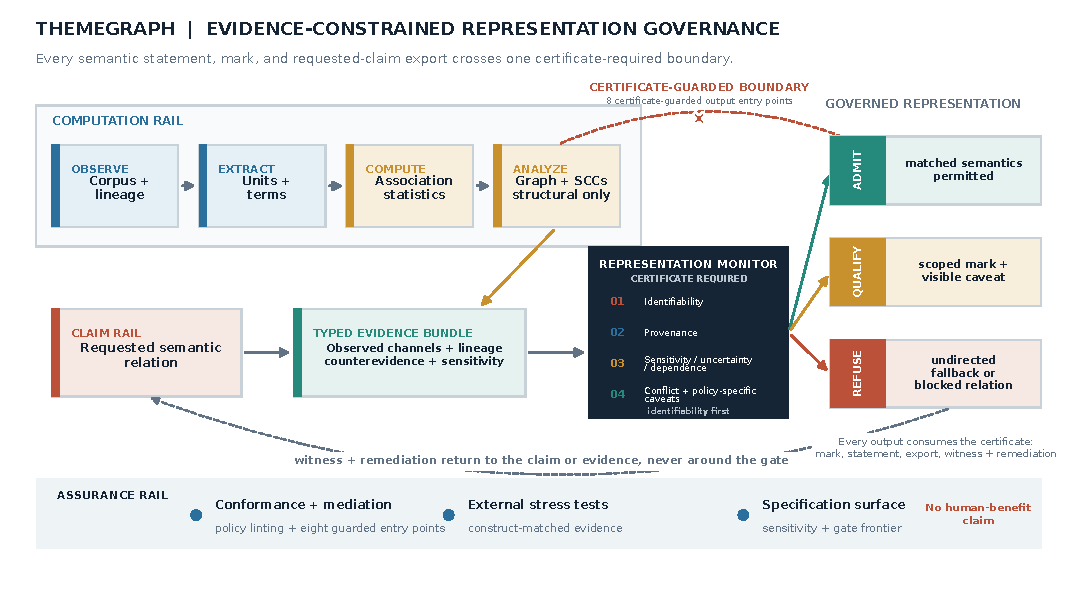
\includegraphics[width=0.98\textwidth]{themegraph_overview_architecture.pdf}
  \caption{Overarching ThemeGraph architecture. A computation rail produces provenance-bearing structural candidates; a separate claim rail combines requested semantics with typed evidence. The maintained inventory has eight certificate-guarded output entry points: two nonsemantic structural serializers require certificate-set integrity, while six semantic representation/export entry points mediate statement, mark, or requested-claim export. The blocked bypass is not a universal future-code assurance or security reference-monitor claim.}
  \Description{A dual-circuit architecture separates corpus-to-graph computation from semantic claim governance. Corpus provenance, deterministic extraction, relation statistics, and graph structure feed a typed evidence bundle. A requested semantic relation and that bundle enter an ordered claim-time policy gate and certificate-required representation monitor. A red blocked bypass prevents direct promotion from graph structure to semantic meaning. Admit, qualify, and refuse certificates govern visible representation and export. An assurance rail contains authored conformance tests, external construct-matched stress tests, a specification surface, and complete-mediation entry-point coverage.}
  \label{fig:overview-architecture}
\end{figure*}

The central methodological demonstration is not that SCCs discover themes. It is that a correct SCC can expose a failure of representation: the cycles are valid for the graph, while the graph's arrows do not warrant the interpretation a viewer could reasonably assign to them.

\section{Related Work}

\subsection{Interpretation and Computational Text Analysis}

Thematic analysis identifies and interprets patterned meaning rather than equating a repeated token pattern with a theme \cite{braun2006}. Reflexive thematic analysis further requires coherence among research question, theoretical assumptions, analytic practice, and claims \cite{braun2021}. ThemeGraph therefore reserves \emph{theme} for human-grounded interpretation and calls graph outputs \emph{structural candidates}. This distinction is constitutive, not cosmetic: replacing the word ``theme'' does not repair an unidentified relation, but it prevents an algorithmic partition from silently inheriting the standing of qualitative interpretation.

Computational approaches can still contribute to interpretive inquiry. Nelson's computational grounded theory uses computation for pattern detection, then returns to human refinement and confirmation \cite{nelson2020}. Topic modeling similarly offers a latent representation of documents \cite{blei2003}, while human evaluation has shown that held-out likelihood and interpretability can diverge \cite{chang2009}. Chuang et al. demonstrate that model-driven text visualization must address interpretation and trust, not only model output \cite{chuang2012}. We extend this lineage with a prior question: does the observation model identify the visualized relation at all? A confidence interval around the wrong construct does not answer that question.

\subsection{Graphs, Association Rules, and Stability}

Association-rule mining introduced support and confidence to describe item co-occurrence \cite{agrawal1993}. A rule $a\rightarrow b$ is directional in its conditional denominator, but that notation does not establish time, cause, prerequisite, discourse, or entailment. Graph algorithms then operate only on the edges supplied to them. Tarjan's depth-first method identifies SCCs in $O(|V|+|E|)$ time \cite{tarjan1972}. Community methods optimize different structural objectives \cite{newman2004}; Leiden, for example, addresses disconnected communities that can arise under Louvain optimization \cite{traag2019}. SCCs, weak components, modularity communities, and vector clusters are therefore not interchangeable theme algorithms. Each answers a different question about a representation.

Stability work offers tools for evaluating sensitivity but does not establish construct validity. Consensus clustering examines agreement under resampling \cite{monti2003}, and stability selection controls selection behavior under subsampling \cite{meinshausen2010}. Specification curve analysis exposes conclusions across defensible analytic choices \cite{simonsohn2020}. These methods motivate distinct policy claims: descriptive persistence over a declared specification set; meeting a declared persistence gate; bootstrap persistence under a declared resampling scheme; and statistical stability under a dependence-aware scheme with adequate uncertainty. The present specification surface supports only the first two. None identifies a different construct: a persistent prevalence-derived arrow remains prevalence-derived.

\subsection{Visualization Expressiveness and Executable Constraints}

APT defines graphical languages for data facts and ranks effective encodings \cite{mackinlay1986}. Draco makes visualization-design knowledge executable as hard and soft constraints \cite{moritz2019}; VizLinter diagnoses and repairs violations in completed visualizations \cite{chen2022}. These systems govern mappings between data, marks, and design rules. ThemeGraph governs a different object: whether a typed evidence bundle is sufficient for the semantics of a requested claim. The decision then changes the graphical language, statement, and export. Thus APT asks whether a visualization expressively represents data facts; Draco and VizLinter operationalize design constraints; ThemeGraph asks whether the available evidence identifies the semantic relation that an otherwise expressive mark would communicate. The mechanisms are complementary, and our novelty claim is limited to policy-declared construct-, object-, and scope-matched claim-time authorization at this semantic representation boundary.

\subsection{Inspectable and Accountable Representations}

Sensemaking and information-foraging accounts connect representations to search, encoding, value, and access costs \cite{russell1993,pirolli1999}. Overview/filter/detail interaction and mixed-initiative principles motivate traversable evidence, user control, and visible state \cite{shneiderman1996,horvitz1999}. Here they provide design rationale, not effectiveness evidence.

Algorithmic contestability requires information, support for contestation, and responsibility attribution \cite{yurrita2025}. ThemeGraph evaluates only a narrower policy-artifact condition: version identity, inspectability, replay, and traceable representational changes.

Representations also distribute cognition across people and artifacts \cite{hutchins1995}. As boundary objects, graph structures may coordinate people with different expertise while retaining different meanings across communities \cite{star1989}. This flexibility is useful but risky when visual syntax suggests more agreement than evidence supports. Uncertainty visualization research likewise shows that evaluation must concern consequences and interpretation, not merely the presence of an uncertainty mark \cite{hullman2019}. Our response is to couple visible uncertainty with a claim decision.

Bolinska argues that successful visual epistemic representation depends on how a representation supports relevant inferences rather than resemblance alone \cite{bolinska2016}. ThemeGraph operationalizes a narrower software criterion without assuming an undefined semantic-strength ordering. For output $o$ and certificate $K$, $\operatorname{Authorized}_v(o,K)=1$ iff the statement belongs to $K$'s permitted statement class, the encoding belongs to its permitted encoding set, and requested-claim exportability permits the attempted export. We define $\operatorname{PolicyConformantRepresentation}_v(o,K)\Leftrightarrow\operatorname{Authorized}_v(o,K)=1$. This criterion establishes consistency with an authored policy, not truth, soundness in a universal epistemic sense, or communicative success.

Provenance represents derivation from inputs and transformations \cite{green2007}; computational argumentation distinguishes support, acceptability, and defeat \cite{dung1995}. Claim-admissibility contracts integrate these established ideas to govern whether graph-derived statements cross into human-facing claims.

\subsection{Construct Validity and Interpretive Fit}

Construct mismatch despite correct computation is established rather than novel. Jacobs and Wallach show how computational operationalizations can fail to correspond to the theoretical constructs a system purports to measure \cite{jacobs2021}. Recent visualization scholarship likewise documents tensions between formal analytic representations and meaning-making in humanities research \cite{benitosantos2026}. ThemeGraph instantiates these concerns at claim time: a versioned policy asks whether the observed evidence type can identify the requested relation before an interface selects its visual grammar. This moves validity reasoning from retrospective documentation into executable, per-claim representation governance. It does not establish that the policy vocabulary is complete or universally correct.

\subsection{Evidence-Gated Runtime Authorization and Promotion Boundaries}

Three neighboring questions must remain distinct. Visualization expressiveness and effectiveness ask whether marks faithfully encode data and whether people can use them. Evidence/state authorization asks whether a claim or action may advance given recorded support and runtime state. ThemeGraph asks whether typed evidence authorizes the \emph{semantic graphical mark and requested-claim export} of a directed text representation.

ResearchLoop treats research questions, evidence objects, claim ledgers, and paper bindings as durable repository-backed state and gates claim admission in AI-assisted research \cite{researchloop2026}. RARE identifies representation-confusion attacks in LLM-assisted reverse engineering; RARE-Guard separates authority from support, groups provenance before support counting, and uses deterministic rendering so downgraded claims do not reappear in reports \cite{rare2026}. FAVA lowers task constraints into evidence-backed permission graphs and uses an SMT authorizer plus runtime gateway before effectful agent actions execute \cite{fava2026}. Proof-or-Stop gates claim-bearing lifecycle transitions on verifiable evidence \cite{prooforstop2026}. CAPAS is public research software that deterministically maps structured scientific claims and evidence to \textsc{Accept}, \textsc{Rewrite}, \textsc{Reject}, or \textsc{Hold} with a replayable audit trail; it governs evidence licensing for controlled scientific-claim reuse while explicitly withholding truth and raw-data-authenticity guarantees \cite{capas2026}. ThemeGraph instead governs the coordinated interactive semantic statement, graph mark, requested-claim export, and projected fallback.

Evidence-Graded Decision Authorization (EGDA) separates clinical evidence extraction, three-level sufficiency assessment, and claim-level authorization through domain-specific rules; authorized outputs are restricted to fact summaries, conditional statements, next-step suggestions, or refusal/deferral \cite{lin2026egda}. Closeness depends on the controlled object and consequence rather than a universal ranking: CAPAS is a deterministic evidence-typed scientific claim-gating and controlled-reuse analogue; EGDA is a pre-output clinical claim/decision-authorization analogue; and claim-specific PCA-biplot admissibility is a scientific-interpretation admissibility analogue because target alignment, spectral identifiability, and projection adequacy govern whether a biplot statement is retained, reformulated, qualified, or rejected \cite{pinto2026}. ThemeGraph's narrower HCI delta is policy-declared construct-, object-, and scope-matched joint control of an interactive graph's semantic statement, mark, requested-claim export, and independently authorized projected fallback. Evidence-gated control planes, promotion boundaries, downgraded rendering, permission graphs, and runtime authorization are not ThemeGraph inventions.

ThemeGraph also adapts an established security architecture intuition. Complete mediation requires authority to be checked on every access, while the classic reference-monitor model requires an always-invoked, non-bypassable mediation point amenable to verification \cite{anderson1972,saltzer1975}. Security reference monitors govern subjects performing operations on protected objects. ThemeGraph governs a different object: a typed claim request over an analytic representation. Its representation monitor maps claim, governed object, evidence, and policy to an admitted, qualified, or refused statement, mark, and requested-claim export. We claim neither invention of complete mediation nor security equivalence; the lineage identifies the non-bypass requirement that Figure~\ref{fig:overview-architecture} applies to semantic output.

\subsection{Claim-Evidence Grounding, Documentation, and Refusal}

PaperTrail decomposes generated scholarly answers and sources into claims and evidence, exposing unsupported assertions and omissions \cite{martinboyle2026}. Its participant study also cautions that greater caution need not change reliance behavior. ThemeGraph addresses a different question: not only whether evidence is linked, but whether the \emph{kind} of evidence can identify the semantics requested from a representation. Model Cards, Datasheets, and AI FactSheets document intended use, lineage, evaluation, and limitations at model, dataset, or service scope \cite{mitchell2019,gebru2021,arnold2019}. Our unit is a requested claim, and the output actively constrains rendering and export rather than remaining passive documentation.

Contemporary work makes evidence sufficiency explicit in other domains. Claim-specific PCA-biplot admissibility is the closest scientific-interpretation admissibility analogue: it asks whether target alignment, spectral identifiability, and projection adequacy support a proposed interpretation, but it does not govern interactive text-graph export \cite{pinto2026}. SURE-RAG distinguishes support, refutation, and insufficiency for selective retrieval-augmented answering \cite{qiu2026}, while REVEAL uses rubrics to identify missing evidence and re-retrieve long-video clues \cite{yan2026}. ClaimDB tests fact verification over large structured databases and emphasizes executable reasoning and abstention when evidence is insufficient \cite{theologitis2026}. MEVER combines graph-based multimodal evidence retrieval, claim verification, and explanation generation \cite{zhang2026mever}. These systems verify or explain claims; ThemeGraph governs a different downstream act: whether a typed claim may be stated, rendered with a particular mark, or exported for a typed object. Verification evidence can feed authorization, but a verified proposition does not by itself authorize every representation, and policy authorization does not establish truth. Table~\ref{tab:prior-art} compares reported mechanisms, not end-to-end systems under a common benchmark or every capability an extension might provide.

Selective prediction defers unreliable predictions and can affect human judgments \cite{bondi2022}; ThemeGraph instead refuses relations that the observations cannot identify. Its demonstrated delta is the conservative alignment of established design, evidence, permission, abstention, and documentation mechanisms at one semantic-output boundary. Table~\ref{tab:prior-art} neither denies adjacent extensibility nor claims novelty for individual components.

Claim-evidence visualization is already inspectable: FaEvR structures fact-evidence reasoning \cite{vaidya2020}; ClaimViz supports factual-claim verification \cite{rony2020}; EvidenceLens, an accepted IEEE VIS 2026 short paper with a preprint available, links financial-QA claims to source passages, cells, and charts \cite{gu2026}; and VAKG models interaction and knowledge provenance \cite{christino2026}. Inspectability explains an output; enforcement governs whether it is permitted. ThemeGraph joins these at a directed graph's semantic-output boundary.

\begin{table*}[t]
  \caption{Representative, non-exhaustive, non-ranking comparison across adjacent design spaces. Closeness depends on controlled object and consequence. Additional systems remain discussed in prose.}
  \label{tab:prior-art}
  \centering
  \footnotesize
  \setlength{\tabcolsep}{2.5pt}
  \begin{tabular}{@{}p{.14\textwidth}p{.15\textwidth}p{.20\textwidth}p{.18\textwidth}p{.24\textwidth}@{}}
    \toprule
    Mechanism & Authorized object & Evidence matching & Decision / consequence & Controlled downstream output \\
    \midrule
    APT / Draco / VizLinter \cite{mackinlay1986,moritz2019,chen2022} & Data fact / visualization specification & Data-fact or design-constraint match & Violation or repair & Design mapping or constraint \\
    PCA admissibility \cite{pinto2026} & Biplot interpretation & Target/operator/projection fit & Retain / reformulate / qualify / reject & Scientific interpretation statement \\
    CAPAS \cite{capas2026} & Structured scientific claim & Evidence-typed admissibility contract & Accept / Rewrite / Reject / Hold & Controlled claim reuse + audit trail \\
    EGDA \cite{lin2026egda} & Clinical claim / action & Evidence grade + domain rules & Fact / conditional / next step / refusal & Clinical language or action output \\
    ResearchLoop \cite{researchloop2026} & Research claim / paper binding & Task contract + evidence object & Claim admission withheld & Paper binding \\
    RARE / RARE-Guard \cite{rare2026} & RE report claim / action & Authority + grouped support & Downgrade or deny & Report rendering / tool promotion \\
    FAVA \cite{fava2026} & Agent action & Evidence/state permission & Counterexample or authorize & Effectful action \\
    ThemeGraph (this work) & Typed text-graph claim & Construct/object/scope predicate & Admit / typed qualify / refuse & Statement + graph mark + requested export + projected fallback \\
    \bottomrule
  \end{tabular}
\end{table*}

No compared system is claimed to lack every component. ThemeGraph's distinction is the controlled object and joint consequence: policy-declared construct, object, and scope matching jointly authorizes, at claim time, an interactive graph's statement, semantic mark, requested-claim export, and any independently justified fallback.

\section{Directed Representation Audit}

\subsection{Observation Model}

Let a corpus contain documents $D$. A deterministic extractor produces text units $U$, such as sentences. Each unit $u$ contains a set of normalized terms $T_u$. Let $N=|U|$, let $n(a)$ be the number of units containing term $a$, and let $n(a,b)$ be the number containing both $a$ and $b$. For nonzero $n(a)$ and $n(b)$, the implemented relation statistics are

\begin{equation}
\operatorname{conf}(a\rightarrow b)=\frac{n(a,b)}{n(a)},
\label{eq:confidence}
\end{equation}

\begin{equation}
\operatorname{lift}(a,b)=\frac{n(a,b)N}{n(a)n(b)}.
\label{eq:lift}
\end{equation}

An ordered edge is retained when its source term and pair supports satisfy minimum counts and both statistics satisfy configured thresholds. The graph includes all eligible vocabulary terms, including isolates and terms that appear only as destinations. Each retained edge stores its statistic values and evidence identifiers.

Figure~\ref{fig:edge-distributions} reports the observed distribution of these statistics on the four corpora the paper claims: synthetic, O*NET, ACM text, and Python standard library. The job-ad workbook that also appears in the pipeline's internal evaluation outputs is excluded from this and every corpus-comparison figure that follows, because its source, sampling frame, and redistribution license are unresolved (Ethics, Limitations, and Scope); the figures therefore match the four-corpus scope already stated for the specification surface.

\begin{figure*}[t]
  \centering
  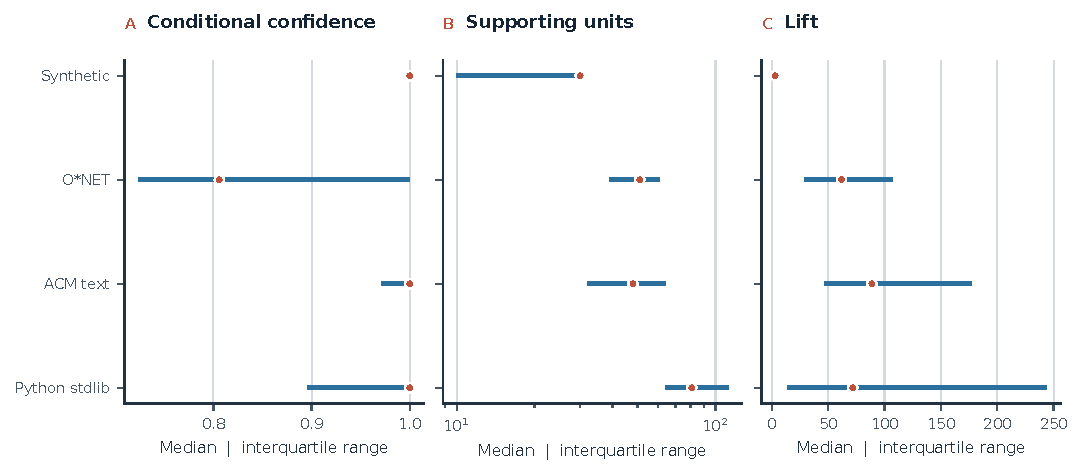
\includegraphics[width=0.92\textwidth]{edge_distributions_core.pdf}
  \caption{Observed conditional confidence, supporting units, and lift for every retained edge in the four corpora this paper claims. Markers are medians and bars are interquartile ranges, read directly from serialized edge records at default configuration; no fitting or smoothing is applied. Supporting units are plotted on a log scale because corpus size varies by four orders of magnitude.}
  \Description{Three panels report the median and interquartile range of conditional confidence, supporting unit count, and lift for the synthetic, O*NET, ACM text, and Python standard library corpora.}
  \label{fig:edge-distributions}
\end{figure*}

The notation in Equation~\ref{eq:confidence} invites a directional reading, but its asymmetry has a simple source:

\begin{equation}
\log\frac{\operatorname{conf}(a\rightarrow b)}{\operatorname{conf}(b\rightarrow a)}
=\log\frac{n(b)}{n(a)}.
\label{eq:identity}
\end{equation}

The joint count cancels. Lift is symmetric. Thus co-occurrence and lift determine whether a pair is eligible, while marginal prevalence determines which conditional confidence is larger. If $n(a,b)=0$, neither confidence ratio nor its logarithm is usable and no supported pair exists. If either marginal is zero, the corresponding confidence and lift are undefined. The implementation avoids these boundary cases by evaluating only observed pairs among supported terms.

Equation~\ref{eq:identity} is elementary probability, not a novel theorem. Its diagnostic consequence is substantial: unordered co-occurrence cannot identify temporal order, syntax, discourse relation, prerequisite, causality, enablement, or semantic hierarchy. Such claims require an additional directional channel.

Figure~\ref{fig:directional-asymmetry} reports the observed magnitude of this identity rather than only its algebra. For every retained edge $a\rightarrow b$, the reverse confidence $\operatorname{conf}(b\rightarrow a)=n(a,b)/n(b)$ is recovered from the same serialized confidence, support, and lift fields via Equations~\ref{eq:confidence} and~\ref{eq:lift}: this is an exact recomputation of already-serialized statistics, not an independent measurement. Median implied reverse confidence is 0.351 for O*NET, 0.468 for ACM text, and 0.206 for Python, each far below the 0.65 admission threshold that the forward orientation met; the planted synthetic corpus, whose core cluster was constructed so its terms co-occur in the same documents, shows little asymmetry (median reverse confidence 1.000, equal to the forward median). The gap in the three real corpora is attributable to the marginal prevalence ratio $n(b)/n(a)$ alone, because support and lift are identical in both orientations; no directional observation distinguishes them.

\begin{figure*}[t]
  \centering
  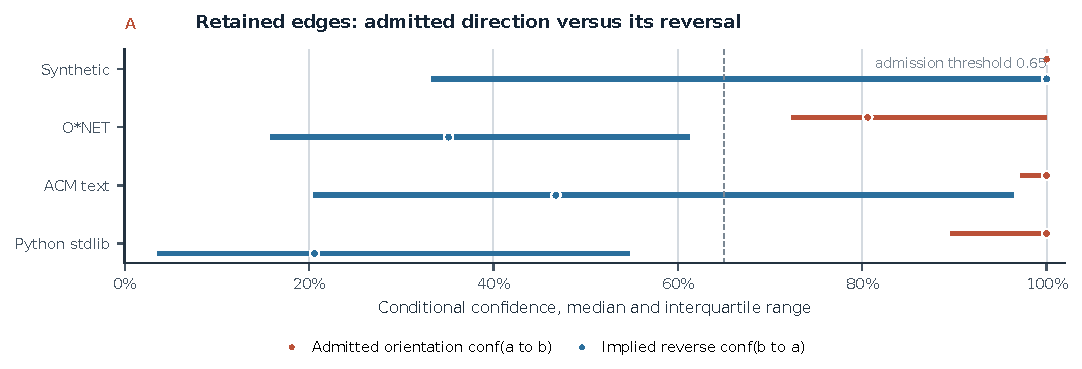
\includegraphics[width=0.92\textwidth]{directional_asymmetry.pdf}
  \caption{Admitted forward confidence against the implied reverse confidence for retained edges in the four claimed corpora, derived from Equations~\ref{eq:confidence} and~\ref{eq:lift}. O*NET, ACM text, and Python show a wide gap between the two orientations; the synthetic corpus does not, because its planted core terms were constructed to co-occur symmetrically. The dashed line marks the 0.65 admission threshold the forward orientation satisfied by construction.}
  \Description{A dumbbell chart compares each corpus's admitted forward confidence, which clusters near one, against the implied reverse confidence, which is far lower for O*NET, ACM text, and Python but similar to the forward value for the synthetic corpus.}
  \label{fig:directional-asymmetry}
\end{figure*}

\begin{table*}[t]
  \caption{Admitted-orientation confidence against the implied reverse-orientation confidence derived from the same serialized support, confidence, and lift fields.}
  \label{tab:directional-asymmetry}
  \centering
  \small
  \begin{tabular}{lrrr}
    \toprule
    Corpus & Retained edges & Admitted conf. median & Implied reverse conf. median \\
    \midrule
    Synthetic & 27 & 1.000 & 1.000 \\
    O*NET & 213 & 0.806 & 0.351 \\
    ACM text & 740 & 1.000 & 0.468 \\
    Python stdlib & 233 & 1.000 & 0.206 \\
    \bottomrule
  \end{tabular}
\end{table*}


Figure~\ref{fig:claim-map} maps the current observation to claims the system may and may not express.

\begin{figure*}[t]
  \centering
  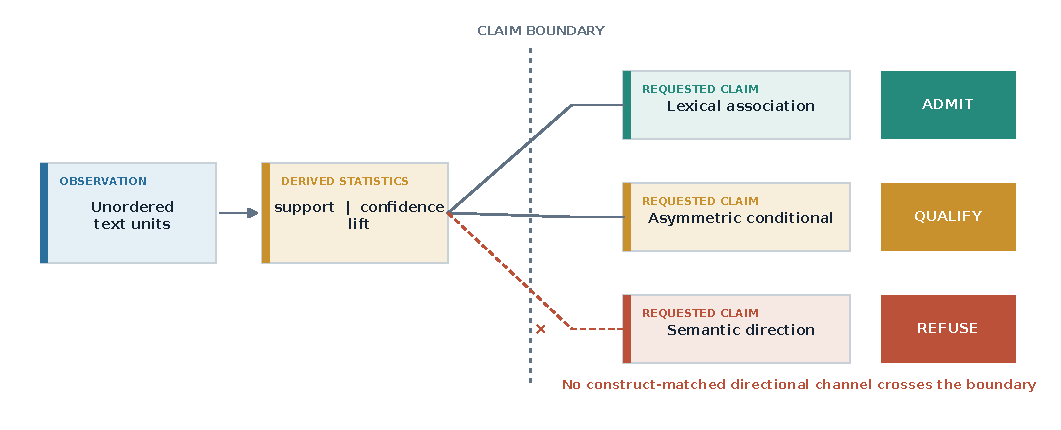
\includegraphics[width=0.94\textwidth]{claim_admissibility_observation_map.pdf}
  \caption{Observation-to-claim mapping for unordered co-occurrence evidence. Lexical association is admitted, asymmetric conditional association is qualified, and semantic direction is refused because no directional evidence channel is observed.}
  \Description{A flow map begins with unordered co-occurrence. It admits lexical association, qualifies asymmetric conditional association as prevalence-dependent, and refuses semantic direction when no directional channel is observed.}
  \label{fig:claim-map}
\end{figure*}

Figure~\ref{fig:dependency-layers} shows the ThemeGraph policy decomposition: computational correctness, construct/evidence admissibility informed where applicable by separately serialized observational-identifiability results, specification robustness, interpretive validity, and human benefit require distinct evidence. Thus $J_g$ and $M_v$ remain separate states rather than one collapsed construct gate. This is a design-specific dependency model, not a universal epistemology.

\begin{figure*}[t]
  \centering
  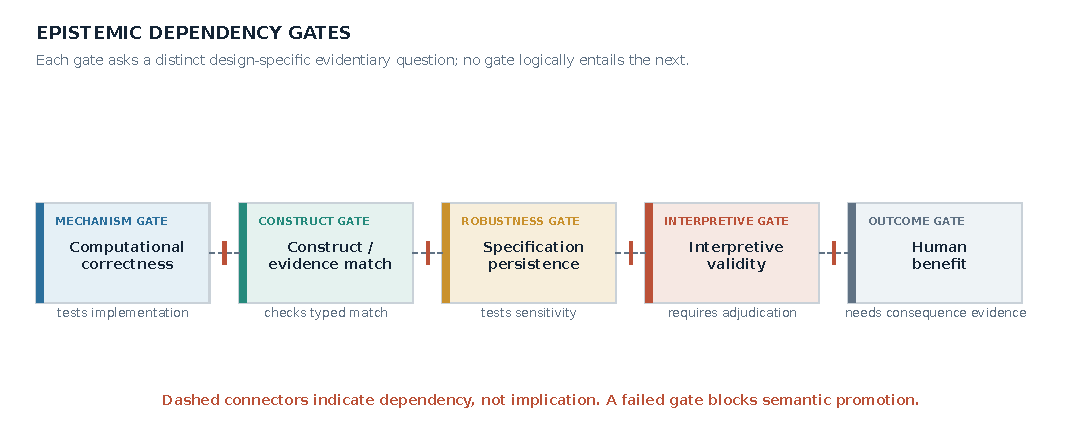
\includegraphics[width=0.96\textwidth]{epistemic_dependency_ladder.pdf}
  \caption{ThemeGraph policy dependency gates. The dependency sequence separates five design-specific evidentiary questions; dashed connectors denote dependency, not logical implication or an ascending epistemological hierarchy.}
  \Description{Five named mechanism, construct, robustness, interpretive, and outcome gates show that computational correctness does not imply construct/evidence match, specification persistence, interpretive validity, or human benefit.}
  \label{fig:dependency-layers}
\end{figure*}

\subsection{Executable Claim-Admissibility Contracts}

We represent a serialized contract as

\begin{equation}
K_v(c,\omega,E_b)=\langle f,c,\omega,\Pi_v,J_g,M_v,O_v,P_{\mathrm{prov}},S,A_u,A_d,C,D_v,H_v,h_v,L_v,R_v,Q_v,X_v,F_v,W_v,\operatorname{Rem}_v\rangle,
\label{eq:contract}
\end{equation}

Operationally, the tuple has three groups: \emph{Inputs} $(f,c,\omega,E_b,\Pi_v)$; \emph{Gate state} $(J_g,M_v,O_v,P_{\mathrm{prov}},S,A_u,A_d,C)$; and \emph{Consequences} $(D_v,H_v,h_v,L_v,R_v,Q_v,X_v,F_v,W_v,\operatorname{Rem}_v)$. This grouping is explanatory and does not change the serialized contract.

where $v$ is policy version; $f$ is one of six claim families; $c$ is a concrete typed claim; $\omega=((a,\tau_a),(b,\tau_b))$ is a governed object; $\Pi_v$ is the policy's evidence-predicate set; and $E_b$ is the complete evidence bundle. $J_g\in\{0,1,\bot\}$ records observational identifiability only where an observation model $g$ supplies a logical result; $\bot$ means not established by this certificate. Complete predicate satisfaction $M_v$ is kept separate from object compatibility $O_v$, provenance $P_{\mathrm{prov}}$, persistence $S$, uncertainty and dependence adequacy $A_u,A_d$, and counterevidence $C$. The ordered evaluator composes these states into $D_v$ and the derived final non-refusal policy-admissibility outcome $\operatorname{PA}_v(c,\omega,E_b)=\mathbf{1}[D_v(c,\omega,E_b)\neq\textsc{Refuse}]$. Serialized \texttt{policy\_admissible} records $\operatorname{PA}_v$ and is omitted from the tuple as an independent state because it is derived rather than a primitive gate. The outcome also includes triggered reasons $H_v$, controlling reason $h_v$, representation authorization $R_v$, and requested-claim export authorization $X_v$. $L_v$ classifies refusal as epistemic, policy, or operational. Statement $Q_v$, fallback $F_v$, witness $W_v$, and remediation $\operatorname{Rem}_v$ make the consequence inspectable. The contract records what an authored policy permits, not truth.

Policy 2.7.0 evaluates structured evidence records rather than channel names alone. Each record is

\begin{equation}
e=\langle x,t,p,\rho_e,m,\mathcal{A},\tau,d,\delta,j\rangle,
\end{equation}

where $x$ is a typed channel, $t$ is its target claim, $p\in\{\mathrm{support},\mathrm{counterevidence}\}$ is polarity, $\rho_e$ is the relation scope to which the record applies, $m$, $\mathcal{A}$, and $\tau$ are method, assumptions, and estimand metadata, $d$ and $\delta$ are study design and diagnostics, and $j\in\{\mathrm{not\mbox{-}reviewed},\mathrm{approved},\mathrm{rejected}\}$ is adjudication status. A predicate $\pi\in\Pi_v(c)$ is evaluated over the complete evidence bundle and governed object, so it may inspect one record or require a conjunction across records. Let $\Sigma_v(c)$ be the claim's permitted source-target type signatures. Object compatibility is

\begin{equation}
O_v(c,\omega)=\operatorname{objectMatch}_{v,c}(\omega)=\mathbf{1}[(\tau_a,\tau_b)\in\Sigma_v(c)].
\label{eq:object-match}
\end{equation}

Complete predicate satisfaction records whether at least one declared predicate is satisfied in full:

\begin{equation}
M_v(c,\omega,E_b)=\mathbf{1}[\exists \pi\in\Pi_v(c):\pi(E_b,\omega)=1].
\label{eq:predicate-identifiability}
\end{equation}

Here $\operatorname{PA}_v=1$ means non-refusal only and therefore includes both \textsc{Admit} and \textsc{Qualify}; it does not authorize every output channel. Statement class $Q_v$, representation set $R_v$, and requested-claim export authorization $X_v$ remain channel-specific, so conflict qualification can be non-refused while ordinary requested-claim export is blocked.

Each $\pi$ includes its declared channel, target, polarity, and scope conditions and, when declared, required record metadata and approved adjudication. Consequently, $M_v$ includes those predicate-local requirements; the evaluator does not reapply them as downstream gates. Serialized adjudication and predicate-metadata fields expose why a predicate did or did not match. Object compatibility $O_v$, provenance $P_{\mathrm{prov}}$, persistence $S$, and uncertainty/dependence adequacy $A_u,A_d$ remain separate gate states. Predicate satisfaction is policy-relative, not proof that assumptions are true. Predicates invoke claim-specific $\operatorname{scopeMatch}_{v,c}(\rho_e,\omega)$. Ordered prerequisite, temporal, entailment, asymmetric-conditional, and causal claims require exact orientation; symmetric lexical association and sentential paraphrase also match reversed pairs. Theme, analyst-benefit, and persistence/stability claims are unscoped. Thus prerequisite evidence must match concept type and orientation; event annotations cannot license term-level temporal requests; and sentence paraphrase annotations cannot license term association. Construct, object type, and orientation are independently necessary.

These checks distinguish schema validity, provenance completeness, and policy-relative predicate satisfaction from upstream semantic correctness/authenticity. In the trust fixture, the source encodes B-before-A; a deliberately faulty adapter emits a schema-valid, provenance-complete A-before-B record, and ThemeGraph authorizes the supplied A-before-B request. The recorded \texttt{semantic\_authenticity\_checked=false} is a diagnostic upstream-assurance annotation, not a Policy 2.7.0 admission gate: it states that this certificate did not independently verify the adapter's semantic faithfulness. The resulting policy conformance is therefore conditional on upstream evidence integrity, not a truth test.

\paragraph{Ordered evaluator.} Policy 2.7.0 executes the following lexicographic decision function; later steps cannot rescue an earlier failed prerequisite.
\begin{enumerate}
  \item Reject an undeclared claim or an object outside $\Sigma_v(c)$; match support and counterevidence by target, polarity, object, and exact scope/orientation.
  \item Record $J_g\in\{0,1,\bot\}$ only from a logical result about observation model $g$. If candidate support relies only on $g$ and $J_g=0$, trigger epistemic refusal. $J_g=\bot$ means that this certificate establishes no such logical result, not automatic permission or refusal.
  \item Evaluate complete predicate match $M_v$ (including any predicate-declared metadata and adjudication requirements), object compatibility $O_v$, persistence, and uncertainty/dependence gates. Do not reapply predicate-local requirements after $M_v$. An independent construct-matched identifying channel may satisfy $M_v$ even when unordered $g$ has $J_g=0$; it does not relabel $g$ as identifying.
  \item Apply provenance and the preceding gate results in declared order. Append every failure to $H_v$ and select the first as $h_v$.
  \item If matched positive support and counterevidence remain, assign reason-specific \textsc{Qualify}; counterevidence alone does not authorize another positive claim unless that distinct claim was requested and matched.
  \item Derive $D_v\in\{\textsc{Admit},\textsc{Qualify},\textsc{Refuse}\}$, then derive only the statement class $Q_v$, mark set $R_v$, and requested-claim export $X_v$ authorized by that certificate.
  \item On refusal, independently evaluate each declared partial projection in $B_v(c)$; select the first target claim whose projected bundle is policy-admissible and provenance-complete, otherwise emit no relation.
  \item Serialize gate state, complete and controlling reasons, output authorization, fallback lineage, witness, and remediation in $K_v$.
\end{enumerate}
The implementation serializes $J_g$ as \texttt{observational\_identifiability}. Its legacy-named \texttt{identifiable} helper/result composes $M_v$, $O_v$, and claim-specific adequacy before the separate provenance check; \texttt{policy\_admissible} records the final non-refusal outcome. Tests cover $J_g=0$, $J_g=\bot$, independent evidence, conflict, gate failure, and fallback independence.

\begin{table}[t]
  \caption{Core notation. Relation scope $\rho_e$ is kept distinct from governed object $\omega$; fallback preferences do not reuse provenance notation.}
  \label{tab:notation}
  \centering
  \small
  \begin{tabular}{@{}lp{.71\columnwidth}@{}}
    \toprule
    Symbol & Meaning \\
    \midrule
    $N$ & Number of extracted text units \\
    $v,f,c,\omega$ & Policy version, claim family, concrete claim, and typed governed object \\
    $\Sigma_v(c),O_v$ & Permitted object signatures and object-match result \\
    $\rho_e$ & Relation scope carried by an evidence record \\
    $E_b,\Pi_v(c)$ & Complete evidence bundle and versioned sufficient predicates \\
    $P_{\mathrm{prov}}$ & Provenance-completeness field \\
    $A_u,A_d$ & Uncertainty and dependence adequacy \\
    $J_g,M_v$ & Observational-identifiability result and complete predicate match \\
    $D_v,\operatorname{PA}_v$ & Decision and derived final non-refusal policy-admissibility outcome \\
    $H_v,h_v,L_v$ & Complete triggered reasons, controlling reason, and refusal class \\
    $R_v,Q_v,X_v$ & Representation authorization, statement, and export authorization \\
    $B_v(c),F_v$ & Ordered fallback preferences and selected fallback \\
    \bottomrule
  \end{tabular}
\end{table}

Policy 2.7.0 organizes fifteen concrete claims into observational, statistical, semantic-relational, causal, interpretive, and human-outcome families (Table~\ref{tab:policy-claim-types}). \textsc{LexicalAssociation} and prevalence-derived \textsc{AsymmetricConditional} are observational. Paraphrase/non-paraphrase, concept equivalence, entailment, temporal precedence, and prerequisite are semantic-relational but retain claim-specific evidence and scope. Four persistence/stability claims are statistical; theme is interpretive; analyst benefit is human-outcome. Causal influence requires an intervention-to-outcome object, a named design, method, assumptions, estimand, diagnostics, \emph{and approved causal adjudication}. These machine-checkable fields establish metadata completeness and routing, not that causal assumptions hold. Intervention remains a design subtype, never an identifying channel by itself. Theme and analyst benefit retain their own approved-adjudication requirements. The present study supplies no causal design, interpretive adjudication, or human evaluation, so these claims remain refused. Policy 2.5.0 replay preserves the earlier metadata-complete but unadjudicated causal behavior; Policy 2.6.0 introduced approved causal adjudication, and active Policy 2.7.0 retains that gate while adding typed fallback projection and complete reason vectors.

\begin{table*}[t]
  \caption{Instantiated Policy 2.7.0 claim types and consequences used in this study.}
  \label{tab:policy-claim-types}
  \centering
  \scriptsize
  \textbf{(a) Families, governed-object signatures, sufficient evidence predicates, and scope semantics}\par\smallskip
  \begin{tabular}{@{}p{.12\textwidth}p{.16\textwidth}p{.15\textwidth}p{.35\textwidth}p{.08\textwidth}@{}}
    \toprule
    Family & Claim type & Object signature & Sufficient bundle predicate & Scope \\
    \midrule
    observational & lexical-association & term->term & co-occurrence & symmetric \\
    observational & asymmetric-conditional & term->term & co-occurrence & ordered \\
    semantic-relational & sentential-paraphrase-equivalence & sentence->sentence & annotation-semantic-equivalence with matched positive paraphrase label & symmetric \\
    semantic-relational & sentential-non-paraphrase & sentence->sentence & annotation-semantic-equivalence with matched non-paraphrase label & symmetric \\
    semantic-relational & concept-equivalence & concept->concept & annotation-semantic-equivalence & symmetric \\
    semantic-relational & textual-entailment & sentence->sentence & annotation-entailment & ordered \\
    semantic-relational & event-temporal-precedence & event->event & event-order OR annotation-temporal-precedence & ordered \\
    semantic-relational & concept-prerequisite & concept->concept & prerequisite-reference OR annotation-prerequisite & ordered \\
    causal & causal-influence & intervention->outcome & causal identification with named design, method, assumptions, target estimand, and diagnostics & ordered \\
    interpretive & theme & analysis->theme-candidate & qualitative interpretation with method, analytic traceability, reflexive documentation, and theory alignment & unscoped \\
    human-outcome & analyst-benefit & interface->analyst-population & human evaluation with outcome, measure, study design, comparator, population, and estimand & unscoped \\
    statistical & specification-persistence & result->specification-surface & specification-surface & unscoped \\
    statistical & meets-specification-persistence-gate & result->specification-surface & specification-surface & unscoped \\
    statistical & bootstrap-persistence-under-declared-scheme & result->resampling-scheme & cluster-bootstrap & unscoped \\
    statistical & statistical-stability & result->resampling-scheme & cluster-bootstrap & unscoped \\
    \bottomrule
  \end{tabular}\par
  \medskip
    \textbf{(b) Representation consequences and lawful fallback projections}\par\smallskip
  \begin{tabular}{@{}p{.16\textwidth}p{.13\textwidth}p{.20\textwidth}p{.14\textwidth}p{.25\textwidth}@{}}
    \toprule
    Claim type & Adjudication & Counterevidence & Encoding & Fallback / projection \\
    \midrule
    lexical-association & not required & qualify-conflict-when-support-matches & undirected-link & none \\
    asymmetric-conditional & not required & qualify-conflict-when-support-matches & conditional-asymmetry-glyph & lexical-association via lexicalize-pair-v1 \\
    sentential-paraphrase-equivalence & not required & qualify-conflict-when-support-matches & undirected-link & lexical-association via lexicalize-pair-v1 \\
    sentential-non-paraphrase & not required & qualify-conflict-when-support-matches & no-relation & none \\
    concept-equivalence & not required & qualify-conflict-when-support-matches & undirected-link & none \\
    textual-entailment & not required & qualify-conflict-when-support-matches & directed-arrow & lexical-association via lexicalize-pair-v1 \\
    event-temporal-precedence & not required & qualify-conflict-when-support-matches & directed-arrow & lexical-association via lexicalize-pair-v1 \\
    concept-prerequisite & not required & qualify-conflict-when-support-matches & directed-arrow & lexical-association via lexicalize-pair-v1 \\
    causal-influence & approved review required & qualify-conflict-when-support-matches & directed-arrow & lexical-association via lexicalize-pair-v1 \\
    theme & approved review required & qualify-conflict-when-support-matches & no-relation & none \\
    analyst-benefit & approved review required & qualify-conflict-when-support-matches & no-relation & none \\
    specification-persistence & not required & qualify-conflict-when-support-matches & no-relation & none \\
    meets-specification-persistence-gate & not required & qualify-conflict-when-support-matches & no-relation & none \\
    bootstrap-persistence-under-declared-scheme & not required & qualify-conflict-when-support-matches & no-relation & none \\
    statistical-stability & not required & qualify-conflict-when-support-matches & no-relation & none \\
    \bottomrule
  \end{tabular}

\end{table*}


Table~\ref{tab:policy-claim-types} is authored Policy 2.7.0, not an independently validated ontology. Its semantic-equivalence channel is claim- and polarity-matched: a positive paraphrase label supports equivalence; a matched non-paraphrase label supports only that separate request and counters equivalence. Extension requires declaring construct/identifier, object signature, scope/polarity/orientation, predicates/proxies, gates, and output/fallback consequences. We exercised extension by adding \texttt{concept-equivalence}, a symmetric concept-pair claim requiring targeted annotation without proxy or fallback. The generic evaluator has no claim-specific branch: valid evidence admits an undirected mark/export, while omitted declaration fails linting. Implemented predicates permit configuration-only claims; new evidence constructs can require validated predicates. This demonstrates schema extensibility, not universal configuration-only support or ontology validity.

Polarity is target-specific. Table~\ref{tab:counterevidence} makes the decision rule explicit. Support with no counterevidence proceeds through downstream gates; matched support plus counterevidence is \textsc{Qualify} with reason code \texttt{conflict-present}; counterevidence without support leaves positive support absent and therefore \textsc{Refuse}. Conflict qualification authorizes an interrupted contested relation and blocks ordinary requested-claim export; it never retains the same solid arrow as \textsc{Admit}. Thus contradiction is not reverse truth, and neither neutral absence nor negative annotation is silently promoted to a different positive relation. Policy-conformant representation is the direct software criterion, not truth or normative policy validity \cite{bolinska2016}.

\begin{table}[t]
  \caption{Support and counterevidence decision rule before downstream gates.}
  \label{tab:counterevidence}
  \centering
  \small
  \begin{tabular}{lll}
    \toprule
    Matched support & Counterevidence & Outcome \\
    \midrule
    No & No & Refuse: insufficient \\
    Yes & No & Continue through gates \\
    No & Yes & Refuse \\
    Yes & Yes & Qualify: conflict \\
    \bottomrule
  \end{tabular}
\end{table}

The encoding \texttt{no-relation} denotes absence of an authorized edge, not a visible assertion that the objects stand in a negative semantic relation. An admitted non-paraphrase statement and a refusal without fallback may therefore both have no edge, while remaining distinct through certificate decision, statement, reasons, witness, and remediation.

Fallback is a versioned policy preference, not a theorem that one claim logically entails another. Policy 2.7.0 lists lexical association as the first supported alternative for specified refused pair-scoped requests only when co-occurrence and lineage are available. A cross-type fallback is lawful only through a declared partial object projection $\phi^v_{c\rightarrow c'}:\Omega_c\rightharpoonup\Omega_{c'}$. The current \texttt{lexicalize-pair-v1} projection is defined only when each endpoint has one canonical lexical handle, both handles map to terms or tokens represented in the corpus, distinct endpoints do not collapse through an identity-changing many-to-one mapping, and the projected pair has independently observed co-occurrence. The projected object uses those handles as its term endpoints while retaining evidence-record and corpus lineage. If any condition fails, the projection is undefined and the consequence is no relation. Let $\phi^v_{c\rightarrow c'\,*}(E_b)$ denote the correspondingly projected bundle. For ordered preferences $B_v(c)$, selection is

\begin{equation}
F_v(c,\omega,E_b)=\operatorname{first}\left\{c'\in B_v(c):
\begin{aligned}
&\phi^v_{c\rightarrow c'}(\omega)\ \text{is defined},\\
&\operatorname{PA}_v\!\left(c',\phi^v_{c\rightarrow c'}(\omega),\phi^v_{c\rightarrow c'\,*}(E_b)\right)=1
\end{aligned}\right\}.
\label{eq:fallback}
\end{equation}

Here $\operatorname{PA}_v$ is the ordered evaluator's complete target decision, including predicate, object, applicable adequacy, counterevidence, and provenance states; it is not $M_v$ alone. The implementation evaluates the projected target through that complete decision. Selection never overrides its $Q_v$, $R_v$, or $X_v$: if the target is \textsc{Qualify}, the fallback inherits its qualified statement, mark, and export restriction rather than appearing as an unqualified substitute. The original refused request remains non-exportable. No fallback is permitted outside the declared preference list, without a declared projection, or when the projected bundle cannot independently authorize the target claim. Thus a refused unscoped theme or analyst-benefit claim does not become a pair-scoped lexical relation, and selecting lexical association does not assert logical implication from the refused semantics. The certificate records target decision and export consequence, projection identifier, source and target claims, projected object, and projection-provenance statements. Version, original object, projected object, and complete lineage remain explicit, so fallback selection is replayable rather than inferred from a channel name.

For a prespecified set of configurations $\Theta$, descriptive specification persistence is

\begin{equation}
S_{\Theta}(r)=\frac{1}{|\Theta|}\sum_{\theta\in\Theta}
\mathbb{1}[r\text{ is produced under }\theta].
\end{equation}

The binary claim that a result meets an authored gate $\gamma$ is separate: $G_{\Theta,\gamma}(r)=\mathbf{1}[S_{\Theta}(r)\geq\gamma]$. Neither $S_{\Theta}$ nor $G_{\Theta,\gamma}$ is a posterior probability. Bootstrap persistence $B_{\mathcal{R}}(r)$ instead reports recurrence under a declared resampling scheme $\mathcal{R}$ that repeats the extraction pipeline. A statistical-stability claim additionally requires a declared criterion, adequate uncertainty, and dependence-aware clustering at the highest defensible independent unit. The current evaluation supplies $S_{\Theta}$ and reports $G_{\Theta,.80}$; it supplies neither $B_{\mathcal{R}}$ nor statistical stability. Unit, document, and source counts remain separate because many sentences can originate from one duplicated document.

\paragraph{Typed Refusal Semantics.} The conservative decision order is important. Missing support, predicate metadata, object compatibility, required adjudication, provenance, or adequacy gates cannot be rescued by later checks. A stable or well-provenanced computation therefore cannot launder a construct mismatch. The certificate distinguishes channel absence, target mismatch, scope mismatch, metadata incompleteness, object mismatch, missing adjudication, persistence-gate failure, uncertainty/dependence inadequacy, conflict, mention-order insufficiency, and incomplete provenance. $H_v$ preserves every triggered reason in policy order while $h_v$ identifies the controlling reason used for the top-level consequence. Refusal is classified as \emph{epistemic} when observations fail to distinguish or support the request, \emph{policy} when an authored requirement is unmet, and \emph{operational} when lineage/export prerequisites are incomplete. \textsc{Qualify} is crossed with its reason: prevalence qualification retains a bar-to-ring statistic, whereas conflict qualification uses an interrupted contested relation and blocks ordinary semantic export. A refused claim may receive a supported lexical fallback, but that fallback does not partially support the refused semantics and $X_v=0$ for the original claim.

Seven adversarial contract properties subject implementation claims to explicit failure tests. \emph{Construct matching} requires target, object signature, and predicate agreement. \emph{No-validity-laundering} states that failure of $M_v$, $O_v$, or any required adequacy or provenance gate implies \textsc{Refuse} regardless of confidence or success on other gates. \emph{Conditional support-channel monotonicity} preserves admission when genuinely admissible support is added unless counterevidence or another failed gate is introduced. \emph{Export conformance} requires every export to satisfy $\operatorname{Authorized}_v$, including $X_v$. \emph{Fallback conformance} requires the fallback to be policy-admissible and first among entries in $B_v(c)$ whose declared projection yields an admissible, provenance-preserving target bundle. \emph{Directional pair-scope non-transfer} prevents evidence for $(a,b)$ from authorizing reversed ordered claim $(b,a)$. Their perturbations and explicit failure conditions form an adversarial contract-property matrix, not epistemological falsification of the authored policy. Policy 2.7.0 is also linted with 21 structural and behavioral checks, including projection completeness and provenance preservation. These checks establish internal consistency, not normative validity or completeness.

\subsection{Observational Equivalence}

\paragraph{Proposition (observational-equivalence refusal).} Let $g$ be an observation function and $r$ a requested latent relation. If admissible worlds $z_1,z_2$ satisfy $g(z_1)=g(z_2)$ but $r(z_1)\neq r(z_2)$, then $r$ is not identifiable from $g$ alone.

\emph{Proof.} Any estimator using only $g$ receives the same input in both worlds and therefore returns the same output, while the requested truth differs. It must be wrong in at least one world unless additional assumptions or observations distinguish them. \hfill$\square$

Consider one world in which alpha precedes beta and another in which beta precedes alpha. After order is discarded, both have marginals $n(\mathrm{alpha})=n(\mathrm{beta})=2$ and joint support $n(\mathrm{alpha},\mathrm{beta})=1$. This established observational-equivalence argument is where ``identifiability'' is warranted: $J_g=0$. ThemeGraph's contribution is making that logical result a machine-checkable representation-refusal trigger. Policy 2.7.0 refuses temporal precedence in both worlds and applies lexical association only when the declared pair projection and fallback evidence independently authorize it. This is a constructive refusal argument, not an uncertainty estimate.

\section{ThemeGraph System}

\subsection{Pipeline and Provenance}

ThemeGraph separates adapters, stable text units, relation extraction, graph analysis, evaluation, and export. Edges retain statistics, document/unit identifiers, and bounded evidence records. Configuration, seed 2027, aggregate-JSON rebuilding, hashes, and source validation support reproducibility; full pipeline and adapter details are supplementary and available at \url{https://github.com/tiamole/themeGraph}, which also hosts the live interactive inspector at \url{https://tiamole.github.io/themeGraph/prototype/}.

That bound is deliberate but has a measurable cost. Each edge's evidence list is capped at three excerpts regardless of how many distinct documents actually support it. Figure~\ref{fig:evidence-retention} reports, for the four claimed corpora, the share of retained edges whose true supporting-document count exceeds that cap. Every retained edge in the synthetic, O*NET, and ACM-text corpora has more supporting documents than the three excerpts shown; Python standard library is lower (65.2\%) because its edges have weaker median document support. This quantifies how much corroborating evidence is withheld from the inspector and from any export by construction; it does not evaluate whether the three shown excerpts are representative of the withheld majority.

\begin{figure*}[t]
  \centering
  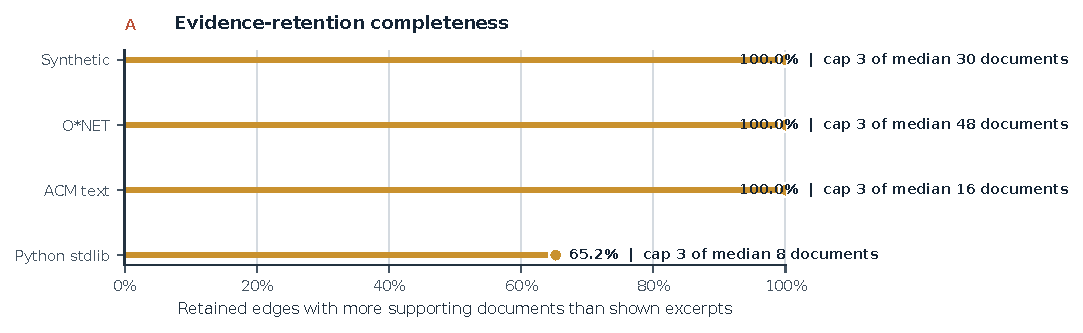
\includegraphics[width=0.8\textwidth]{evidence_retention.pdf}
  \caption{Share of retained edges, across the four claimed corpora, whose evidence list is truncated because the number of distinct supporting documents exceeds the serialized cap of three excerpts, with the median number of supporting documents annotated for each corpus.}
  \Description{A dot plot reports the share of retained edges whose supporting-document count exceeds the three-excerpt evidence cap for the synthetic, O*NET, ACM text, and Python standard library corpora, annotated with the median number of supporting documents in each corpus.}
  \label{fig:evidence-retention}
\end{figure*}

\begin{table*}[t]
  \caption{Share of retained edges whose supporting-document count exceeds the serialized evidence cap of three excerpts.}
  \label{tab:evidence-retention}
  \centering
  \small
  \begin{tabular}{lrrr}
    \toprule
    Corpus & Retained edges & Share truncated & Median supporting documents \\
    \midrule
    Synthetic & 27 & 100.0\% & 30 \\
    O*NET & 213 & 100.0\% & 48 \\
    ACM text & 740 & 100.0\% & 16 \\
    Python stdlib & 233 & 65.2\% & 8 \\
    \bottomrule
  \end{tabular}
\end{table*}


The maintained implementation imposes a complete-mediation requirement over the currently inventoried output boundary. Its eight certificate-guarded output entry points fail closed on missing, duplicate, unknown, malformed, or inconsistent certificate state. Two nonsemantic structural serializers (analysis-result serialization and CLI structural export) require complete certificate-set integrity. Six semantic representation/export entry points (the governed-representation and requested-claim APIs, inspector statement/mark/export rendering, and publication enforcement) consume a selected certificate. Witness and remediation are certificate-derived fields rendered through certificate-bound inspector/API state, not additional independently selectable semantic emitters. The validator derives colocated declarations, checks each guard, and rejects an unlisted synthetic emitter; this bounded discovery is not proof over arbitrary future code.

The core contains no corpus-specific vocabulary or graph rule and executes unchanged across the evaluated source types. This is dataset independence as an engineering claim, not construct validity or transportability of meaning.

\subsection{Graph Computation and Complexity}

The extractor deduplicates terms per unit, counts unordered pairs, evaluates both conditional orientations, and applies iterative Tarjan SCC extraction in $O(|V|+|E|)$ \cite{tarjan1972}; pair counting costs $O(\sum_u k_u^2)$. Further invariants are supplementary, and correctness does not authorize semantics.

\subsection{Inspector Prototype}

The static inspector accepts a requested claim, corpus, and filters; its certificate determines statement, graph mark, and export. The complete interface exposes typed evidence, gate state, reasons, fallback, witness, and remediation, while Figure~\ref{fig:inspector-policy27} retains the decision-critical fields. Policy 2.7.0 maps lexical association to an undirected link, prevalence qualification to a bar-to-ring glyph, conflict qualification to an interrupted mark with blocked ordinary export, and admitted semantic direction to a solid arrow (Figure~\ref{fig:governance-grammar}). Refusal emits only an independently admissible projected fallback or no relation. Components remain structural candidates, not validated themes, and these marks are unvalidated design assignments.

Figure~\ref{fig:inspector-policy27} uses a causal refusal whose lexical projection is undefined, so it emits no fallback; it is distinct from Table~\ref{tab:claim-benchmark}'s \texttt{unsupported-causality} bundle, whose canonical lexical handles, represented terms, observed pair, and retained lineage independently satisfy the declared lexical fallback projection.

\begin{figure*}[t]
  \centering
  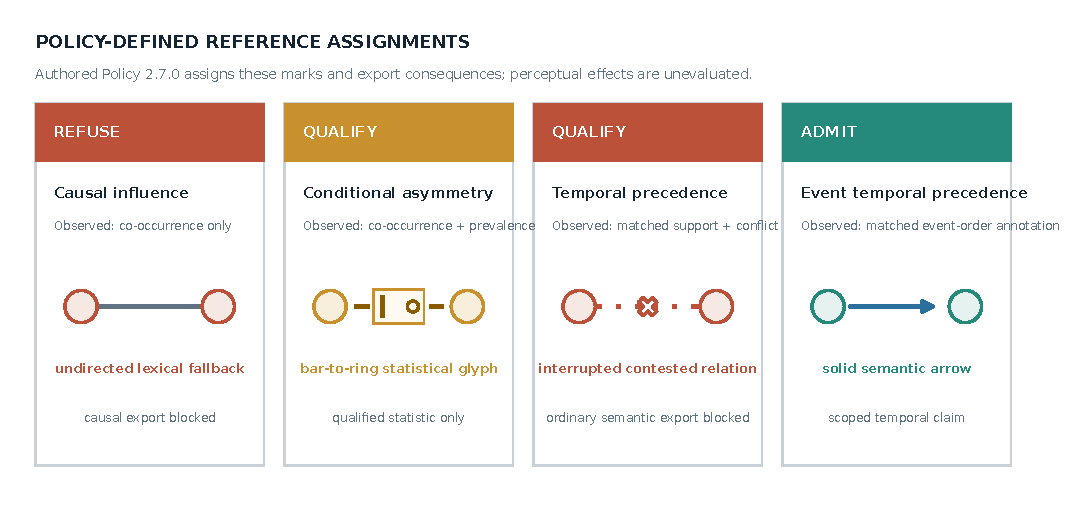
\includegraphics[width=0.98\textwidth]{governance_state_triptych.pdf}
  \caption{Policy-defined reference assignments under authored Policy 2.7.0. \textsc{Refuse} blocks causality and permits only a projection-backed undirected lexical fallback; prevalence \textsc{Qualify} uses a bar-to-ring statistic; conflict \textsc{Qualify} uses an interrupted contested relation and blocks ordinary semantic export; \textsc{Admit} alone permits a solid semantic arrow. These are unvalidated design assignments, not confidence levels or demonstrated perceptual encodings.}
  \Description{Four side-by-side states show refused causality with lexical fallback, prevalence-qualified conditional asymmetry with a bar-to-ring glyph, conflict-qualified temporal precedence with an interrupted line and conflict marker, and admitted temporal precedence with a solid arrow.}
  \label{fig:governance-grammar}
\end{figure*}

\begin{figure*}[t]
  \centering
  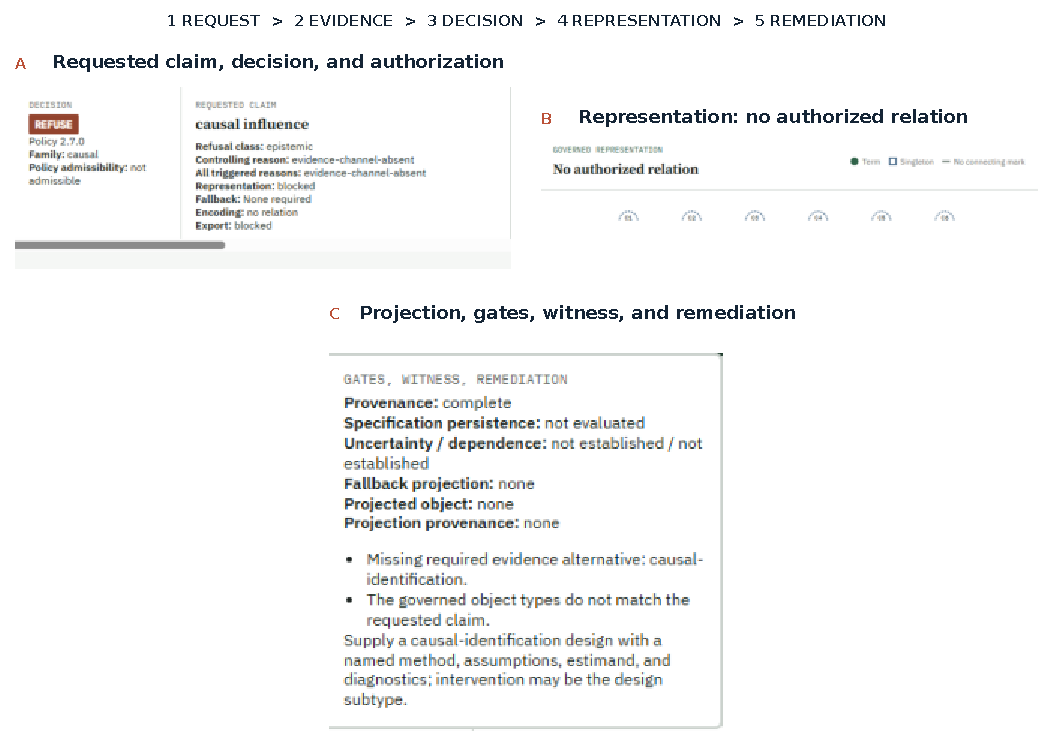
\includegraphics[width=0.98\textwidth]{inspector_policy27_composite.pdf}
  \caption{Policy 2.7.0 decision-critical inspector composite, organized as Request, Evidence, Decision, Representation, Remediation. Panel A shows the requested causal claim, observed evidence, refusal, controlling reason, blocked export, and absent fallback; Panel B shows the certificate-governed no-relation encoding; Panel C enlarges projection, gate, witness, and remediation fields. The complete inspector remains in the artifact. This verifies implementation visibility and sequence, not usability, perceptual effectiveness, or benefit.}
  \Description{Three annotated inspector panels show a refused causal request with its observed evidence and controlling reason, an empty graph because no edge is authorized, and enlarged projection, gate, witness, and remediation fields. The empty graph does not assert a negative semantic relation.}
  \label{fig:inspector-policy27}
\end{figure*}

\section{Mechanism Evaluation}

\subsection{Research Questions}

We ask five mechanism questions, labeled RQ1a, RQ1b, RQ2, RQ3, and RQ4. RQ1a: across the declared adversarial fixtures and currently inventoried certificate-guarded output boundary, does the executable policy conform to declared decisions, reasons, marks, exports, fallbacks, object signatures, scope, and invariants, and does enforcement control reachable representations? RQ1b: can policy linting detect targeted faults, and do versioned changes produce traceable consequences? RQ2: over MRPC and PAWS, do construct-matched paraphrase and non-paraphrase labels exercise the declared routes, including high-overlap negatives? RQ3: across SNLI entailment, AL-CPL prerequisite direction, and TORQUE temporal precedence, does pair-matched evidence authorize only its annotated construct and orientation while insufficiency, counterevidence, mention order, reversal, and cross-construct requests follow declared paths? RQ4: how do lexical associations and components change across a bounded specification surface and alternative persistence gates?

Four stages evaluate conformance, representational enforcement, external construct boundaries, and specification robustness. RQ1a spans Stages 1 to 2; RQ1b uses Stage 1; RQ2 to RQ3 use Stage 3; and RQ4 uses Stage 4. Human interpretation and benefit remain future Stages 5 to 6.

\subsection{Evaluation Logic and Evidentiary Scope}

ThemeGraph is evaluated as a participant-free representation-governance mechanism. Authored cases test evaluator-policy agreement; adversarial properties and mutations test invalid transfer, override, projection, and export rules; representation fixtures test output consequences; the eight-entry boundary audit tests certificate or certificate-set integrity; and replay tests attributable policy-version differences. External labels test construct-, object-, scope-, polarity-, and direction-bounded routing, while the specification surface tests change under bounded analytic choices. These are mechanism tests, not predictive, truth, stability, or human-effect evaluations.

This logic instantiates Figure~\ref{fig:dependency-layers}. Stages 1 to 2 answer RQ1a to RQ1b through conformance, fault detection, policy replay, and representation enforcement; Stage 3 answers RQ2 to RQ3 through construct-bounded routing; Stage 4 answers RQ4 through descriptive specification sensitivity. Perceptual effectiveness, usability, trust, calibration, unsupported-inference reduction, analyst performance, and benefit require distinct human-consequence evidence. The external corpora remain bounded: SNLI entailment does not validate temporal or prerequisite direction; AL-CPL prerequisites do not validate temporal precedence; and TORQUE event order does not validate prerequisite or causal influence.

\subsection{Policy Conformance Testing}

Ten authored cases compare declared decisions, reasons, fallbacks, witnesses, and representations with serialized Policy 2.7.0 certificates; disagreement would expose evaluator-policy divergence. Seven executable properties probe invalid construct or scope transfer, unsupported semantic override, fallback leakage, and export leakage. Twenty-one targeted mutations ask whether malformed declaration, evidence typing, adjudication, projection, representation/export, or versioning rules survive linting. Row-level triggers remain in the artifact. These tests establish implementation-policy conformance and fault localization, not normative validity.

A certificate-guarded output-entry-point audit derives all eight declarations and checks their boundary. Focused tests require exactly one selected certificate where applicable, reject missing/unknown claims and malformed decision/mark combinations, and block refused exports. Browser and publication validators check certificate consistency, source equality, every declared guard, and unlisted synthetic emitters. This is bounded source and behavior coverage, not formal non-bypassability proof.

Replay makes two policy boundaries concrete: reversing a prerequisite pair changes admission under target-only Policy 2.2.0 to refusal under pair-scoped Policy 2.7.0, while causal admission under Policy 2.5.0 becomes adjudication-dependent in Policies 2.6.0 to 2.7.0. Certificates retain policy version and behavioral witnesses; patch versions must preserve decisions, representations, and export authorization. Later policy is inspectable, not presumed superior.

Two controlled fixtures complete this stage. Observationally equivalent opposing temporal worlds retain identical unordered signatures. Four co-occurrence-only prerequisite requests are refused, then admitted after exactly pair-matched prerequisite records are added. These are mechanism checks; AL-CPL provides the separate annotated prerequisite stress test.

\subsection{Output-Control Reachability Ablation}

The ablation holds graph/evidence inputs, governed object, requested claim, and requested semantic output specification constant; only whether certificate consequences control rendering/export changes. Three generated fixtures request: (1) temporal precedence from co-occurrence alone, with an authorized lexical fallback; (2) temporal precedence with matched support and counterevidence, requiring conflict qualification; and (3) lexical association with incomplete provenance, requiring refusal without fallback.

Four generated output-control conditions use each fixture: graph-pipeline-only emits requested outputs without certificate-visible control; warning-layer adds a non-controlling warning; certificate-visible-non-enforcing exposes the certificate without changing reachability; ThemeGraph enforcement derives outputs from it. Counts inspect statement, semantic mark, requested-claim export, and lawful fallback. \emph{Reachable} means emitted, selectable, renderable, or exportable as an output under that condition/fixture; a fallback merely mentioned in certificate metadata is excluded. \emph{Unauthorized} means not authorized under Policy 2.7.0 for that fixture. This three-fixture ablation is separate from the eight-entry-point audit, not a $3\times8$ cross-product, human/performance comparison, safety proof, or characterization of all warning systems.

\subsection{External Construct-Matched Policy Stress Testing}

External labels exercise only their published constructs, and aggregate relations are not independent samples. MRPC contributes 5,801 paraphrase judgments \cite{dolan2005}; PAWS-Wiki contributes 65,401 high-overlap pairs \cite{zhang2019}. Co-occurrence alone must refuse paraphrase equivalence; positive annotation may support it; a negative label counters that claim and supports only a separately requested non-paraphrase claim. Jaccard summaries stress this boundary rather than classifier accuracy.

SNLI contributes 569,033 premise-hypothesis labels \cite{bowman2015}: entailment supports only its observed direction, neutral is insufficient, contradiction is counterevidence, and reversal receives no transfer. AL-CPL contributes 6,529 processed concept pairs, including 2,002 positive prerequisites \cite{liang2018,wang2016}, normalized prerequisite $\rightarrow$ target; absent row-level origin flags preclude attributing individual pairs to preprocessing operations. TORQUE contributes 1,928 public adjudicated-development event relations \cite{ning2020}; 184 directional questions without answer indices and withheld test answers are excluded. It exercises matched temporal admission, mention-order insufficiency, reversal, and cross-construct refusal.

\subsection{Specification Surface}

We evaluate 24 equally weighted deterministic configurations for ACM text, O*NET, Python standard-library text, and the planted corpus. Eighteen vary unitization, features, capacity, vocabulary, support, confidence, lift, or deduplication singly; six add bounded two-factor stresses. This is not an exhaustive or weighted multiverse.

For union edges and nontrivial SCCs, we report intersection, alternatives, exact persistence, and default similarity. One-to-one maximum-weight Jaccard matching prevents reuse of an observed component. Union and default gate frontiers span 0.50, $2/3$, 0.75, 0.80, 0.90, and 1.00; 0.80 is an authored heuristic, not a truth probability. Full configurations and exclusions remain in Table~\ref{tab:specification-surface} and the artifact package.

\subsection{Corpora and Configuration}

The four views are 90 planted documents, descriptions/tasks from the first 500 O*NET 30.3 occupations \cite{onet303}, 18 ACM template files, and 100 Python files; the latter three are mechanics corpora, not substantive populations. A separate dependence check repeats 12 generated records four times. The optional workbook audit remains outside the paper's claims.

Defaults are a 500-term cap, confidence 0.65, and lift 1.05; the threshold grid crosses confidence 0.50/0.65/0.80 with lift 1.00/1.05/1.25. Values were prespecified, not optimized for a preferred component.

Figure~\ref{fig:corpus-structure} compares the four corpora's default-configuration structure, and Figure~\ref{fig:measured-performance} reports single-environment execution cost. Both are read directly from \texttt{research\_evaluation\_summary.json} and share the four-corpus scope stated above.

\begin{figure*}[t]
  \centering
  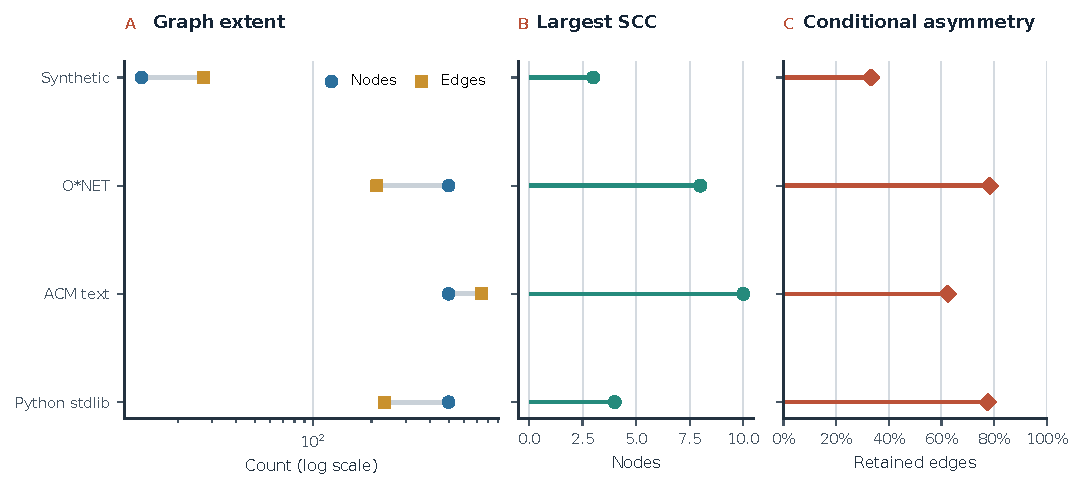
\includegraphics[width=0.92\textwidth]{cross_corpus_structure_core.pdf}
  \caption{Default-configuration structural extent across the four claimed corpora. Panel A compares vocabulary size (nodes) and retained edges on a log scale; panel B reports the largest strongly connected component; panel C reports the share of retained edges that are asymmetric, meaning only one orientation passed the confidence and lift thresholds. Corpora differ by more than an order of magnitude in vocabulary size yet show no consistent relationship between corpus size and largest-component size.}
  \Description{Three panels compare node and edge counts on a log scale, largest strongly connected component size, and the share of asymmetric retained edges across the synthetic, O*NET, ACM text, and Python standard library corpora.}
  \label{fig:corpus-structure}
\end{figure*}

\begin{figure*}[t]
  \centering
  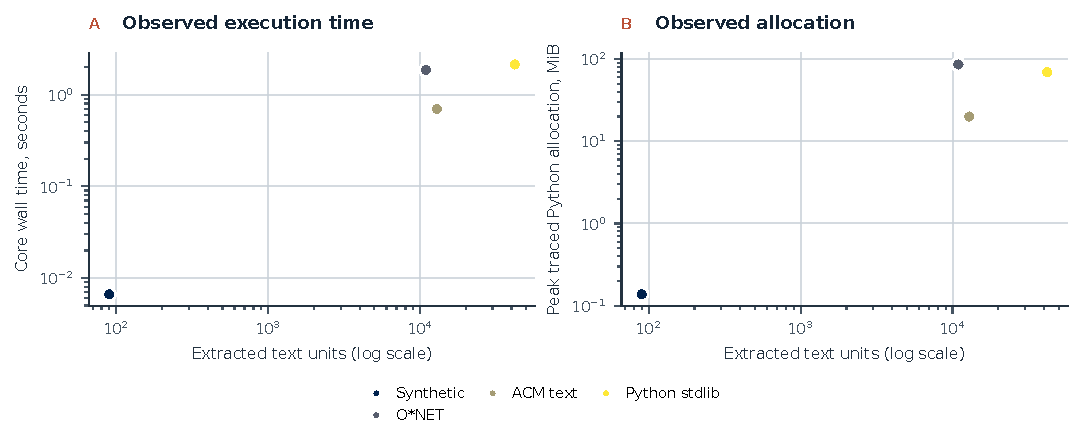
\includegraphics[width=0.92\textwidth]{measured_performance_core.pdf}
  \caption{Observed single-environment wall-clock time and peak traced Python allocation against extracted text units, on log-log axes, for the four claimed corpora (recorded environment: Python 3.14.0, Windows-11). These are single-run observations on one machine, not a controlled benchmark across repetitions, hardware, or competing implementations; they bound expected cost on the evaluated corpora, not asymptotic complexity.}
  \Description{Two log-log scatter plots show core wall time and peak Python allocation increasing with the number of extracted text units across the synthetic, O*NET, ACM text, and Python standard library corpora.}
  \label{fig:measured-performance}
\end{figure*}

\subsection{Baselines, Measures, and Validation}

Baselines cover weak/symmetrized/singleton structure, modularity, seeded Louvain, reversal, and three clustering methods on the planted-core features. ARI, pairwise measures, structural sensitivity, and single-environment runtime/allocation observations do not support an SCC-superiority claim.

Correctness tests compare exact SCC partitions with NetworkX across isolates, destination-only nodes, reversal, symmetrization, and acyclicity. Publication scripts validate deterministic rebuilds, hashes, source equality, formats, and bibliography-aware compilation.

\section{Results}

\subsection{Policy Conformance and Representation Consequences}

All ten controlled cases produced their declared decision and fallback (Table~\ref{tab:claim-benchmark}). Decision and fallback disagreements were zero, and every non-admitted case received remediation. The regenerated table reports observed evidence separately from the complete reason vector and controlling reason, exact witness, and remediation: present-but-inadequate evidence is no longer mislabeled as absent. These results show that Policy 2.7.0 behaves as authored, not that the policy is externally or normatively valid.

\begin{table*}[t]
  \caption{Policy decisions, complete typed reasons, and representation consequences in the controlled benchmark; all observed decisions equal their authored expectations.}
  \label{tab:claim-benchmark}
  \centering
  \scriptsize
  \setlength{\tabcolsep}{1.2pt}
  \begin{tabular}{@{}p{.10\textwidth}p{.10\textwidth}p{.055\textwidth}p{.10\textwidth}p{.10\textwidth}p{.13\textwidth}p{.09\textwidth}p{.055\textwidth}p{.20\textwidth}@{}}
    \toprule
    Controlled case & Requested claim & Decision & Observed evidence & Controlling reason & All triggered reasons & Representation & Export & Exact witness \\
    \midrule
    unordered-association & lexical-association & ADMIT & co-occurrence & none & none & undirected-link & allowed & All gates passed \\
    prevalence-asymmetry & asymmetric-conditional & QUALIFY & co-occurrence & prevalence-qualification & prevalence-qualification & conditional-asymmetry-glyph & allowed & Prevalence-derived orientation \\
    unsupported-temporal-order & event-temporal-precedence & REFUSE & co-occurrence & evidence-channel-absent & evidence-channel-absent & undirected-link & blocked & Missing event-order evidence \\
    observed-temporal-order & event-temporal-precedence & ADMIT & co-occurrence, event-order & none & none & directed-arrow & allowed & All gates passed \\
    explicit-prerequisite & concept-prerequisite & ADMIT & co-occurrence, prerequisite-reference & none & none & directed-arrow & allowed & All gates passed \\
    unsupported-causality & causal-influence & REFUSE & co-occurrence, mention-order, syntax & evidence-channel-absent & evidence-channel-absent & undirected-link & blocked & Missing causal-identification evidence \\
    low-specification-persistence & meets-specification-persistence-gate & REFUSE & co-occurrence, specification-surface & persistence-gate-failed & persistence-gate-failed & no-relation & blocked & S=0.650 < gate=0.800 \\
    duplicated-evidence & statistical-stability & REFUSE & cluster-bootstrap & uncertainty-inadequate & uncertainty-inadequate, dependence-inadequate & no-relation & blocked & Uncertainty inadequate; dependence resampling absent \\
    conflicting-annotations & event-temporal-precedence & QUALIFY & annotation-temporal-precedence & conflict-present & conflict-present & contested-relation & blocked & Opposing matched temporal annotations \\
    missing-lineage & lexical-association & REFUSE & co-occurrence & provenance-incomplete & provenance-incomplete & no-relation & blocked & Required provenance incomplete \\
    \bottomrule
  \end{tabular}
\end{table*}


The representation-enforcement fixture instantiates five certificate states: admission, prevalence qualification, conflict qualification, refusal with fallback, and refusal without fallback (Table~\ref{tab:representation-enforcement}). In every state, the generated statement, semantic mark, requested-claim export result, fallback, witness, and remediation match the declared certificate consequence. In particular, conflict blocks ordinary requested-claim export despite retaining a contested statement, and refusal never emits the requested semantic arrow. This verifies executable state-to-representation coupling for the five fixtures; it does not establish that people perceive or use the marks as intended.

\begin{table*}[t]
  \caption{Certificate-to-representation enforcement under Policy 2.7.0.}
  \label{tab:representation-enforcement}
  \centering
  \scriptsize
  \setlength{\tabcolsep}{1.2pt}
  \begin{tabular}{@{}p{.12\textwidth}p{.06\textwidth}p{.12\textwidth}p{.12\textwidth}p{.12\textwidth}p{.07\textwidth}p{.10\textwidth}p{.07\textwidth}p{.08\textwidth}p{.06\textwidth}@{}}
    \toprule
    Certificate state & Decision & Controlling reason & Permitted statement & Mark & Export & Fallback & Witness & Remediation & Conforms \\
    \midrule
    admit & ADMIT & none & semantic claim & directed-arrow & allowed & none & present & none & yes \\
    prevalence-qualify & QUALIFY & prevalence-qualification & qualified statistic & conditional-asymmetry-glyph & allowed & none & present & present & yes \\
    conflict-qualify & QUALIFY & conflict-present & contested claim & contested-relation & blocked & none & present & present & yes \\
    refuse-with-fallback & REFUSE & evidence-channel-absent & fallback statement & undirected-link & blocked & lexical-association & present & present & yes \\
    refuse-without-fallback & REFUSE & evidence-channel-absent & refusal explanation & no-relation & blocked & none & present & present & yes \\
    \bottomrule
  \end{tabular}
\end{table*}


The Output-Control Reachability Ablation applies three fixtures to four generated output-control conditions (Table~\ref{tab:architecture-ablation}). Each non-enforcing condition leaves three policy-relative unauthorized statements, marks, and exports reachable; visibility alone changes none. Enforcement emits none and preserves one authorized lexical fallback. Separately, all eight currently inventoried certificate-guarded output entry points pass their audit; no $3\times8$ cross-product is claimed. The ablation isolates enforcement, not general warning, human, safety, or noninterference effects.

\begin{table*}[t]
  \caption{Output reachability for three generated adversarial fixtures under four output-control conditions. Unauthorized means not authorized under Policy 2.7.0 for the supplied claim/evidence fixture. Each numeric entry is a count out of the three fixtures. A fallback only listed in certificate metadata is not reachable unless emitted, selectable, renderable, or exportable as an output. The ablation isolates enforcement: it does not compare human effectiveness or characterize all warning or inspection systems. Eight maintained certificate-guarded output entry points are audited separately, not as a 24-case cross-product.}
  \label{tab:architecture-ablation}
  \centering
  \scriptsize
  \begin{tabular}{@{}p{.25\textwidth}rrrr@{}}
    \toprule
    Output-control condition & Statements & Marks & Exports & Fallbacks \\
    \midrule
    graph-pipeline-only & 3/3 & 3/3 & 3/3 & 0/3 \\
    warning-layer & 3/3 & 3/3 & 3/3 & 0/3 \\
    certificate-visible-non-enforcing & 3/3 & 3/3 & 3/3 & 0/3 \\
    themegraph-certificate-enforcement & 0/3 & 0/3 & 0/3 & 1/3 \\
    \bottomrule
  \end{tabular}
\end{table*}


The observational-equivalence test produced identical unordered signatures for worlds with opposing latent temporal directions. Both temporal claims were refused and both returned lexical association as fallback. This directly demonstrates the no-validity-laundering property: equal provenance, support, confidence, lift, and specification behavior cannot repair evidence that has discarded the distinguishing observation.

All seven executable contract-property checks passed (Figure~\ref{fig:contract-properties}). In particular, a sentence-to-sentence paraphrase annotation did not identify event-to-event temporal precedence, complete persistence and uncertainty fields did not rescue unsupported causality, refused requested claims remained non-exportable, every emitted fallback followed its declared object- and scope-compatible preference list, and forward prerequisite evidence did not identify the reversed pair. Figure~\ref{fig:contract-properties} exposes the perturbation and failure condition for each property, stating how each implementation claim could fail rather than presenting pass labels alone. Passing these checks establishes internal conformance of the tested policy paths only.

The typed-contract necessity ablation removes or corrupts each of seven contract distinctions and exposes cross-object licensing, orientation transfer, counterevidence promotion, lineage loss, silent fallback, refused-export leakage, or promotion without adjudication (Table~\ref{tab:contract-field-necessity}). We selected distinctions that directly control cross-construct or cross-object transfer, downgrade provenance, required adjudication, or semantic-output permission. Other serialized fields remain important for diagnosis, replay, or accountability; their exclusion from this probe does not show them unnecessary. Each selected probe is detected, establishing implementation-specific necessity rather than an exhaustive or ontologically minimal contract.

\begin{table*}[t]
  \caption{One-at-a-time contract-field removals and corruptions with their reachable invalid behavior; these probes establish implementation necessity, not ontological minimality.}
  \label{tab:contract-field-necessity}
  \centering
  \scriptsize
  \begin{tabular}{@{}p{.16\textwidth}p{.38\textwidth}p{.28\textwidth}p{.05\textwidth}@{}}
    \toprule
    Removed distinction & Invalid behavior enabled & Joint-control consequence & Detected \\
    \midrule
    governed-object type & Sentence evidence may license an incompatible event or concept claim. & Object-specific authorization collapses into channel-only admission. & yes \\
    scope and orientation & Evidence for a->b may license b->a. & Directional authorization transfers to an unevidenced pair. & yes \\
    evidence polarity & A negative annotation may be read as positive support or reverse truth. & Construct conflict becomes an admitted semantic relation. & yes \\
    projection provenance & A fallback may lose lineage while remaining emit-able. & The downgraded representation is no longer auditable to its evidence. & yes \\
    fallback projection & A refused semantic claim may silently collapse to lexical association. & Refusal no longer controls the representation reached by downgrade. & yes \\
    export authorization & A visibly refused claim may leak into a downstream artifact. & Statement and mark governance can be bypassed through export. & yes \\
    required adjudication & Metadata-complete causal evidence may be promoted without approval. & An authored governance gate disappears while the claim still admits. & yes \\
    \bottomrule
  \end{tabular}
\end{table*}


Table~\ref{tab:architecture-ablation} tests why enforcement matters for generated reachability; Table~\ref{tab:contract-field-necessity} tests why typed enforcement matters in this implementation. Removing object, orientation/scope, polarity, projection lineage, fallback, export, or adjudication distinctions exposes different invalid outputs. This is not a superiority claim over every simpler gate.

In the trust-boundary fixture, source truth is B-before-A, while a faulty adapter supplies a schema-valid, provenance-complete A-before-B record and request. Policy 2.7.0 admits A-before-B, demonstrating conformance conditional on upstream semantic integrity; \texttt{semantic\_authenticity\_checked} remains false.

The version-comparison cases make contestability concrete. Reversed prerequisite evidence changes from \textsc{Admit} under target-only Policy 2.2.0 to \textsc{Refuse} under Policy 2.7.0 pair scope. Metadata-complete but unadjudicated causality changes from \textsc{Admit} under Policy 2.5.0 to \textsc{Refuse} with \texttt{adjudication-required} under Policy 2.7.0. Serialized certificates preserve version, governed object, complete and controlling reasons, witness, projection provenance, and remediation. All 21 active-policy lint checks pass, and all 21 targeted invalid policies trigger their intended checks. The supplementary mutation artifact reports all six families and retains every row, intended check, observed trigger vector, and co-trigger. This assurance is not independent policy validation.

Figure~\ref{fig:policy-lint-mutations} reports the full 21-by-21 trigger matrix behind this count. Fifteen of 21 mutations localize to exactly their intended invariant; the remaining six also trip one or two further invariants. Removing the claim declaration additionally trips interpretive adjudication required; the unreachable-predicate and duplicate-predicate mutations each additionally trip interpretive adjudication required and interpretive metadata consistent; the fallback-cycle and unscoped-to-pair-fallback mutations each additionally trip fallback projections complete; and the undeclared-fallback-target mutation additionally trips all claims declared. This reports which checks co-trigger, not why; it does not explain the covariance and is not an exhaustive guarantee against unanticipated policy faults.

\begin{figure*}[t]
  \centering
  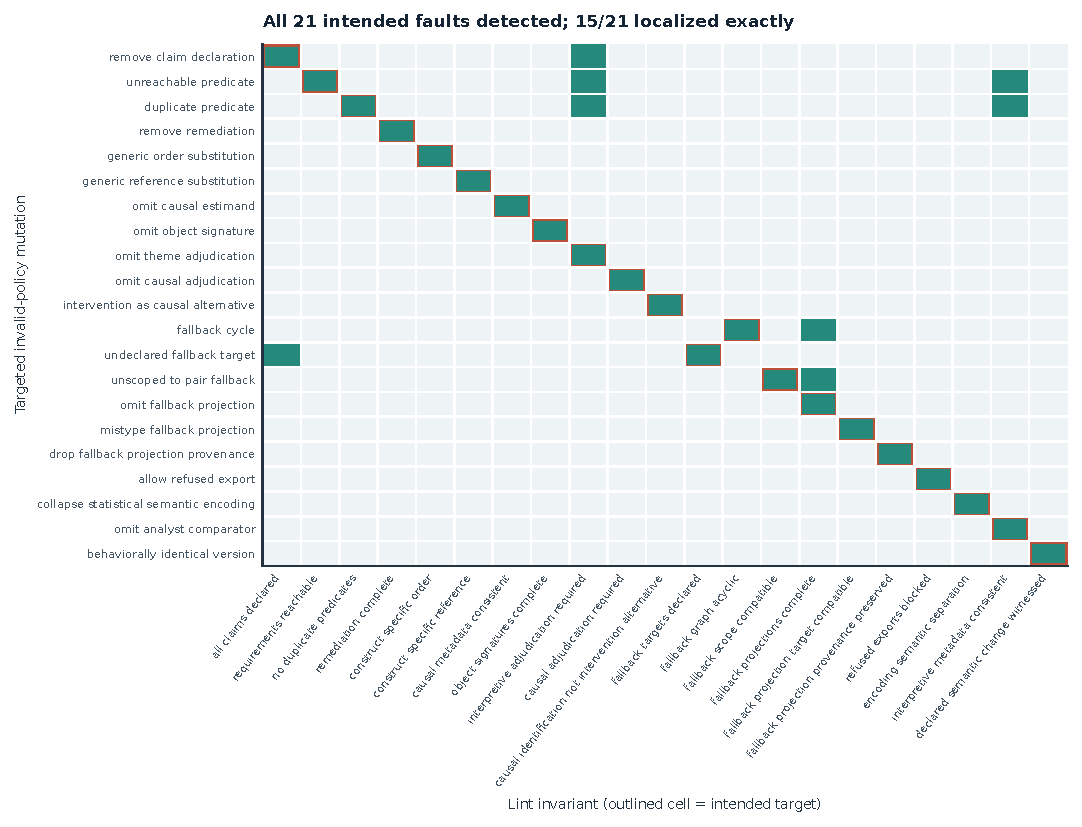
\includegraphics[width=0.92\textwidth]{policy_lint_mutations.pdf}
  \caption{Observed trigger matrix for the 21 targeted Policy 2.7.0 lint mutations against the 21 lint invariants. Outlined cells mark each mutation's intended target; filled cells report which invariants it actually triggered. All 21 intended faults are detected, and 15 of 21 mutations trigger no invariant beyond their intended target.}
  \Description{A 21 by 21 grid marks which lint invariant each targeted mutation triggers; outlined cells show the intended target, and six rows additionally trigger one or two further invariants beyond their intended target.}
  \label{fig:policy-lint-mutations}
\end{figure*}

\begin{figure*}[t]
  \centering
  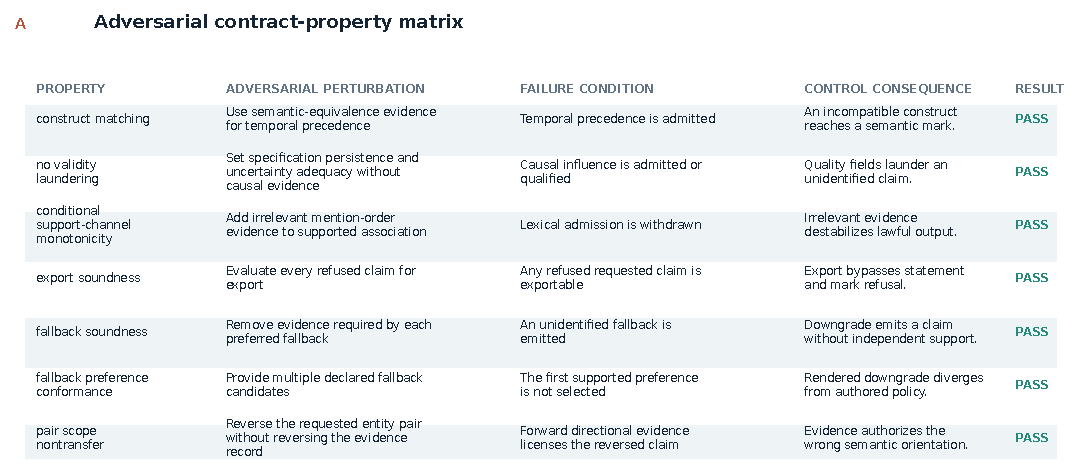
\includegraphics[width=0.88\textwidth]{contract_properties.pdf}
  \caption{Adversarial contract-property matrix under Policy 2.7.0. Each row states a perturbation, the implementation failure it could expose, its consequence for joint output control, and the observed conformance result; this is invariant testing, not epistemological falsification of the policy.}
  \Description{A seven-row matrix lists each policy property, adversarial perturbation, failure condition, control consequence, and pass result, including ordered-pair non-transfer.}
  \label{fig:contract-properties}
\end{figure*}

The evidence-transition fixture refused all four prerequisite requests under co-occurrence alone. After adding the four exactly matched prerequisite-bearing reference records, all four followed the declared admission path. The permitted representation consequently changed from an undirected fallback to a directed prerequisite relation. The supplementary figure preserves the full transition. Because the references are synthetic and perfectly parsed, this result tests policy transition and representation coupling only; it does not establish performance on real references.

\subsection{External Construct-Boundary Stress Tests}

Five datasets exercise paraphrase, entailment, prerequisite, and temporal routes (Table~\ref{tab:external-validation}). Results are organized by failure mode; observed agreement is policy conformance, not predictive performance or independent validation.

\paragraph{Lexical evidence is not semantic evidence.} MRPC and PAWS lexical-only routes refused paraphrase equivalence, whereas positive construct-matched annotation admitted it and negative annotation refused it; separately requested non-paraphrase claims admitted under their own matched scope. Yet 558 of 1,901 MRPC non-paraphrases (29.4\%) and 36,492 of 36,497 PAWS non-paraphrases (99.99\%) exceed Jaccard 0.5. The five PAWS exceptions prevent a universal claim, while the observed high-overlap negatives provide empirical counterexamples to lexical overlap as generic paraphrase evidence. SNLI likewise contains 15,415 neutral and 9,542 contradictory pairs with Jaccard at least 0.5.

\paragraph{Directional evidence does not transfer by reversal.} SNLI premise-to-hypothesis entailment admitted only in its annotated orientation; neutral pairs lacked support, contradictions supplied counterevidence, and reversal refused. AL-CPL admitted matched prerequisite orientation but refused mention order, counterevidence, and reversal. Its processed labels contain no reflexive positive or positive reverse; every positive has a dataset-provided negative, and positives close 1,356 observed two-edge compositions. Without row-level origin flags, these are structural properties, not reconstruction of preprocessing. TORQUE's 1,928 usable adjudicated-dev relations admitted under pair-matched temporal annotation, while mention order and reversal refused; withheld test answers were not evaluated.

\paragraph{Construct-matched evidence does not transfer across constructs.} Cross-construct admission was zero in all five datasets: SNLI entailment did not authorize prerequisite or temporal claims, AL-CPL prerequisites did not authorize temporal claims, and TORQUE event order did not authorize prerequisites. Compact table rows aggregate concrete typed requests rather than inventing pseudo-claims. Artifact JSON retains every requested claim, deterministic request count, expected and observed consequence, policy version, and stable route ID. These diverse routes stress the authored boundaries; they do not establish policy validity, universal relation truth, or excluded constructs.

\begin{table*}[t]
  \caption{Deterministic construct-boundary Policy 2.7.0 transition map. Rows show evidence condition, requested claim, expected and observed policy consequences, and the exercised failure or authorization path; they are conformance routes, not predictive accuracy estimates. Cross-construct rows compact exact typed requests retained with counts and route IDs in the artifact manifest.}
  \label{tab:external-validation}
  \centering
  \scriptsize
  \begin{tabular}{@{}p{.07\textwidth}p{.16\textwidth}p{.15\textwidth}p{.08\textwidth}p{.08\textwidth}p{.24\textwidth}@{}}
    \toprule
    Dataset & Evidence condition & Requested claim & Expected & Observed & Failure / authorization path \\
    \midrule
    MRPC & matched positive annotation & sentential-paraphrase-equivalence & ADMIT & ADMIT & authorized \\
    MRPC & lexical evidence only & sentential-paraphrase-equivalence & REFUSE & REFUSE & missing construct-matched evidence \\
    MRPC & negative annotation & sentential-paraphrase-equivalence & REFUSE & REFUSE & construct-matched counterevidence \\
    MRPC & matched non-paraphrase annotation & sentential-non-paraphrase & ADMIT & ADMIT & authorized \\
    MRPC & cross-construct request & multiple excluded typed claims; see artifact manifest & REFUSE & REFUSE & construct mismatch \\
    PAWS & matched positive annotation & sentential-paraphrase-equivalence & ADMIT & ADMIT & authorized \\
    PAWS & lexical evidence only & sentential-paraphrase-equivalence & REFUSE & REFUSE & missing construct-matched evidence \\
    PAWS & negative annotation & sentential-paraphrase-equivalence & REFUSE & REFUSE & construct-matched counterevidence \\
    PAWS & matched non-paraphrase annotation & sentential-non-paraphrase & ADMIT & ADMIT & authorized \\
    PAWS & cross-construct request & multiple excluded typed claims; see artifact manifest & REFUSE & REFUSE & construct mismatch \\
    SNLI & matched directional annotation & textual-entailment & ADMIT & ADMIT & authorized \\
    SNLI & neutral annotation & textual-entailment & REFUSE & REFUSE & insufficient support \\
    SNLI & contradiction annotation & textual-entailment & REFUSE & REFUSE & construct-matched counterevidence \\
    SNLI & reversed relation request & textual-entailment & REFUSE & REFUSE & scope mismatch \\
    SNLI & cross-construct request & multiple excluded typed claims; see artifact manifest & REFUSE & REFUSE & construct mismatch \\
    AL-CPL & matched prerequisite annotation & concept-prerequisite & ADMIT & ADMIT & authorized \\
    AL-CPL & lexical evidence only & concept-prerequisite & REFUSE & REFUSE & missing construct-matched evidence \\
    AL-CPL & mention order only & concept-prerequisite & REFUSE & REFUSE & evidence-channel-absent \\
    AL-CPL & negative annotation & concept-prerequisite & REFUSE & REFUSE & construct-matched counterevidence \\
    AL-CPL & reversed relation request & concept-prerequisite & REFUSE & REFUSE & scope mismatch \\
    AL-CPL & cross-construct request & multiple excluded typed claims; see artifact manifest & REFUSE & REFUSE & construct mismatch \\
    TORQUE & matched event-order annotation & event-temporal-precedence & ADMIT & ADMIT & authorized \\
    TORQUE & mention order only & event-temporal-precedence & REFUSE & REFUSE & mention-order-insufficient \\
    TORQUE & reversed relation request & event-temporal-precedence & REFUSE & REFUSE & scope mismatch \\
    TORQUE & cross-construct request & multiple excluded typed claims; see artifact manifest & REFUSE & REFUSE & construct mismatch \\
    \bottomrule
  \end{tabular}
\end{table*}


Figure~\ref{fig:external-validation} derives a dataset-by-route-family coverage matrix from the authoritative route records and preserves seventeen representative policy paths. Table~\ref{tab:external-validation} additionally reports separately requested non-paraphrase admission and the remaining cross-construct controls.

\begin{figure*}[t]
  \centering
  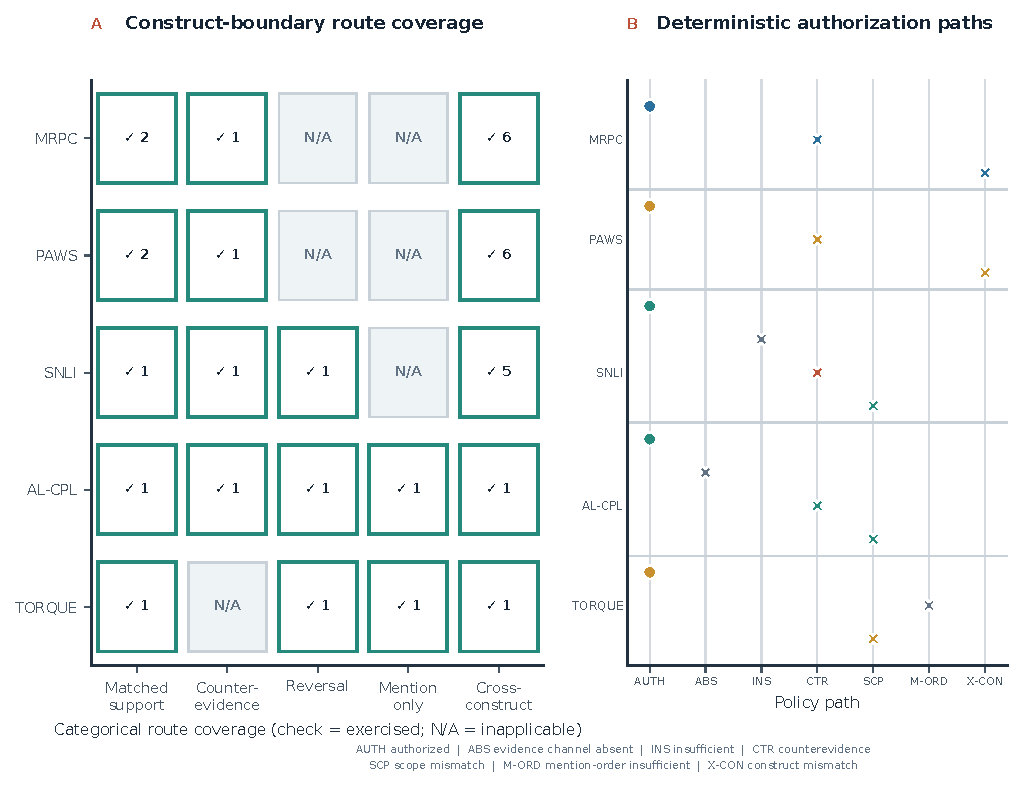
\includegraphics[width=0.92\textwidth]{external_validation.pdf}
  \caption{External construct-boundary Policy 2.7.0 routing map. Left: categorical source-derived coverage of matched support, counterevidence, reversal, mention-only, and cross-construct route families; checks carry route counts, N/A marks inapplicable families, and counts are not independent observations. Right: seventeen deterministic policy paths. Neither panel reports predictive accuracy.}
  \Description{A five-dataset categorical coverage matrix uses outlined cells, checks with source-derived counts, and N/A labels beside seventeen deterministic authorization and refusal paths. Circles mark authorization; crosses locate channel absence, insufficiency, counterevidence, scope mismatch, mention-order insufficiency, or construct mismatch.}
  \label{fig:external-validation}
\end{figure*}

\subsection{Specification Persistence}

Across 24 configurations, the ACM-text union contains \TGAcmtUnionEdges{} edges (Table~\ref{tab:specification-surface}; Figure~\ref{fig:specification-survival}). Default-edge mean persistence is \TGAcmtDefaultMeanPersistence{}; the intersection has \TGAcmtIntersectionEdges{} edges; and mean one-to-one component Jaccard is \TGAcmtComponentJaccard{}. At the authored 0.80 persistence gate, \TGAcmtAuthorizedEdges{} union edges meet the gate and \TGAcmtQualifiedEdges{} fall below it. The union denominator exposes selection hidden by default-only persistence.

O*NET has no edge in the 24-way intersection and 9 of 3,520 union edges meet the 0.80 persistence gate; Python has 135 of 1,063. All 27 default synthetic edges persist throughout, but 120 alternatives emerge below the gate. This reflects the planted core, not general robustness. Analytic choices alter both retention and the candidate universe.

Figure~\ref{fig:threshold-sensitivity} isolates the confidence-by-lift grid underlying this sensitivity. At every tested confidence level, moving lift from 1.00 to 1.25 leaves the largest strongly connected component and the retained edge count unchanged in all three corpora shown; confidence alone drives the response. This follows from lift's symmetry (Equation~\ref{eq:lift}): because the admitted edges in these three corpora already satisfy lift well above 1.25 once they satisfy confidence 0.50, the lift gate is non-binding across this grid. The tested range does not establish that lift is uninformative in general, only that it does not bind here.

\begin{figure*}[t]
  \centering
  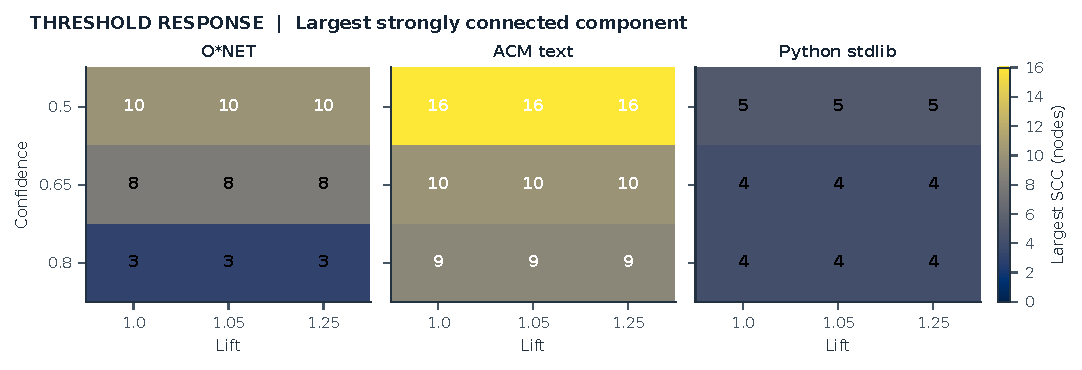
\includegraphics[width=0.85\textwidth]{threshold_sensitivity_core.pdf}
  \caption{Largest strongly connected component across the full prespecified confidence by lift grid for O*NET, ACM text, and Python standard library; the synthetic corpus is omitted because its planted-core component structure does not change across this grid. Lift produces no change at any fixed confidence level in any of the three corpora.}
  \Description{Three heatmaps show the largest strongly connected component size at each combination of confidence and lift threshold for O*NET, ACM text, and Python standard library, with lift producing no change at fixed confidence.}
  \label{fig:threshold-sensitivity}
\end{figure*}

\begin{table*}[t]
  \caption{Union-edge persistence, set geometry, and one-to-one component overlap over an unweighted 24-configuration surface including six bounded interactions; the final columns report outcomes relative to the prespecified 0.80 persistence gate.}
  \label{tab:specification-surface}
  \centering
  \small
  \setlength{\tabcolsep}{1.2pt}
  \begin{tabular}{lrrrrrrrrrr@{}}
    \toprule
    Corpus & Cfg. & 2-factor cfgs. & Default & Union & Min. & Mean & Default mean & 1:1 comp. J & Meets pers. gate & Below pers. gate \\
    \midrule
    ACM text & 24 & 6 & 740 & 9118 & 0.042 & 0.115 & 0.798 & 0.756 & 289 & 8829 \\
    O*NET & 24 & 6 & 213 & 3520 & 0.042 & 0.088 & 0.711 & 0.663 & 9 & 3511 \\
    Python stdlib & 24 & 6 & 233 & 1063 & 0.042 & 0.226 & 0.814 & 0.776 & 135 & 928 \\
    Synthetic & 24 & 6 & 27 & 147 & 0.042 & 0.248 & 1.000 & 1.000 & 27 & 120 \\
    \bottomrule
  \end{tabular}
\end{table*}


\begin{figure*}[t]
  \centering
  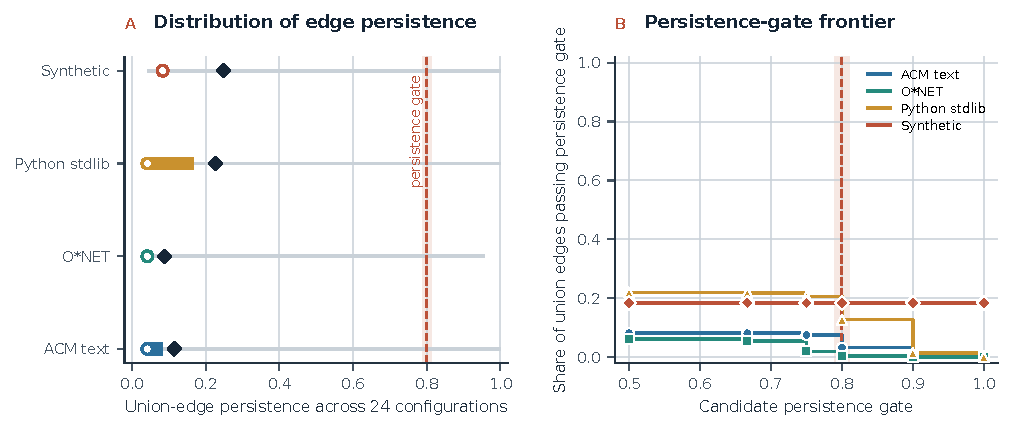
\includegraphics[width=0.92\textwidth]{specification_survival.pdf}
  \caption{Union-edge persistence and persistence-gate frontiers across the unweighted 24-configuration surface. Markers are evaluated gates; connecting steps do not imply interpolated measurements. The dashed 0.80 line is an author-specified heuristic, not a truth threshold.}
  \Description{The left panel compares union-edge persistence across ACM, O*NET, Python, and synthetic corpora. The right panel shows the share of each union passing the authored persistence gate as it moves from 0.50 to 1.00.}
  \label{fig:specification-survival}
\end{figure*}

These consequences remain subordinate to construct evidence and policy admissibility. A persistent lexical association cannot be upgraded to temporal, prerequisite, or causal direction without the corresponding evidence and policy requirements. Conversely, a low-persistence but explicitly referenced prerequisite may be qualified for sensitivity rather than refused for missing semantic evidence. The readable top-level \textsc{Qualify} is crossed with typed reasons: $S=.042$ is highly specification-sensitive, $S=.792$ is near threshold, and construct conflict receives a different mark and export consequence. The gates answer different questions and are intentionally lexicographic.

\subsection{Supporting Correctness and Dependence Checks}

The SCC implementation exactly matched NetworkX across canonical and seeded fixtures, including isolate, destination-only, acyclicity, reversal, and symmetrization invariants. On the easy planted core, SCC and all three clustering baselines obtained ARI and pairwise F1 of 1.0, precluding an SCC-superiority claim. Complete supporting results remain in the artifact package.

The controlled dependence sanity check uses no third-party text. Repeating 12 generated source records four times produces 48 rows, 36 duplicates beyond first occurrence, and the predetermined mechanical consequence that row-level support is four times source-level support. This is a controlled counterexample to equating rows with independent evidence; it is not a substantive empirical finding or a general estimate of dependence in text corpora. Full fixture values remain in the supplementary artifact package.

\section{Discussion}

\subsection{The Arrow Is a Claim, Not a Decoration}

The central implication is representational. A pipeline can pass unit tests, preserve provenance, produce stable identifiers, and render mechanically valid graphics while still using an arrow that exceeds its observations. Conventional software validation asks whether the implementation matches the specification. Claim admissibility asks whether the specification licenses the statement a person is invited to infer. For interactive systems, enforcing that decision at the visible-and-exportable boundary is an HCI capability: it changes which semantic objects the interface can present and propagate, not merely which caveat a backend records.

This distinction changes interface design. A legend that says ``confidence'' is insufficient because readers may reasonably interpret direction semantically. A tooltip with a source sentence is insufficient because the sentence establishes co-occurrence, not direction. A high lift value is insufficient because lift is symmetric. A cycle is insufficient because SCCs are invariant under global reversal. Refusal must therefore govern the representation, not merely annotate it: a refused arrow becomes an undirected fallback or no relation, the requested semantic statement is not exportable, and the interface states what evidence could change the decision.

Claim-admissibility contracts provide such an account without another scalar trust score. A certificate separates observational identifiability, policy admissibility, typed reason, refusal class, representation authorization, and export authorization. Conflict receives a contested mark and blocked ordinary export, not an admitted arrow. Versioning makes requirements inspectable and replayable without changing earlier certificates.

Refusal is actionable only when its cause is preserved: epistemic refusal calls for construct-matched evidence, policy refusal for satisfying or contesting an authored gate, and operational refusal for repairing lineage or output prerequisites. Reason-specific qualification distinguishes prevalence, sensitivity, and conflict. Refusal does not authorize downgrade; fallback must independently earn its representation, otherwise the system emits no relation. These are mechanism principles, not additional contributions.

\subsection{What the Current Evidence Establishes}

The four present stages establish bounded mechanism claims. Stage 1 establishes computational correctness and conformance to author-specified Policy 2.7.0 examples, properties, replay boundaries, and targeted lint mutations. Stage 2 establishes that the tested certificate fields control the implemented statement, mark, fallback, and export. Stage 3 establishes declared routes for construct-, object-, pair-, and direction-matched external annotations and counterexamples. Stage 4 establishes descriptive sensitivity over the declared specification surface. Observational equivalence adds a logical result: the tested unordered signature cannot distinguish opposing temporal worlds.

Evidence beyond authored case agreement carries the main discriminating weight: observational equivalence establishes a non-identification result; typed-field removals expose distinct invalid outputs; the faulty-adapter fixture separates policy conformance from source truth; external high-overlap negatives challenge lexical evidence transfer; the specification surface exposes analytic-choice sensitivity; and mutation plus entry-point audits test the maintained output boundary.

These results do not establish predictive accuracy, independent sampling, universal relation truth, normative policy validity, causal truth, theme validity, perceptual effectiveness, usability, trust, calibration, reduced unsupported inference, improved analytic judgment, or analyst benefit. MRPC, PAWS, SNLI, AL-CPL, and TORQUE exercise only their released constructs and processed labels. The specification surface establishes neither bootstrap persistence nor dependence-aware statistical stability and does not calibrate truth. This boundary is substantive: the present contribution is an executable control capability and a prerequisite for evaluating human consequences, not evidence that those consequences occur.

Supporting negative results constrain interpretation. Perfect synthetic recovery did not distinguish SCC from clustering baselines, and default structure varies across choices and duplicate handling. Temporal, prerequisite, and causal direction remain unidentified in unordered graph corpora; AL-CPL and TORQUE are separate policy probes, not evidence that co-occurrence acquired those semantics. ThemeGraph withholds each relation unless its requirements are met.

These findings also refine what ``dataset-independent'' means. The architecture accepts heterogeneous corpora without core-code changes, which is useful research-software evidence. The outputs remain dataset-dependent, as they should. Cross-domain execution is not transportability of meaning. A contract makes this distinction concrete by separating an engineering check from a construct claim.

\subsection{Implications for CHI Constituencies}

The mechanism evaluation supports three bounded design propositions. First, Tables~\ref{tab:representation-enforcement} and~\ref{tab:contract-field-necessity}, together with the entry-point audit, motivate treating a semantic mark as a consequence-bearing claim surface whose statement, encoding, and export share authorization. Second, Table~\ref{tab:representation-enforcement}, Equation~\ref{eq:fallback}, and the refusal/fallback fixtures motivate reason-specific, repair-oriented refusal that identifies what failed, what representation remains admissible, and what evidence could change the outcome without silently promoting a fallback. Third, policy replay and mutation tests motivate treating executable policy as an inspectable and contestable interaction object whose version, requirements, and representational consequences can be compared. These propositions connect visualization, human-AI interaction, qualitative analysis, and research-software governance without claiming measured human benefit.

\subsection{Reusable Implementation Principles}

Five design principles derived from ThemeGraph's mechanism evaluation may transfer beyond this prototype while remaining testable at the mechanism level:
\begin{enumerate}
  \item \textbf{Guard semantic claim surfaces.} Jointly authorize statements, marks, and requested-claim exports; each inventoried semantic entry point consumes a valid certificate, and a computed edge cannot directly select a semantic arrow.
  \item \textbf{Separate identification from policy.} Record what observations can distinguish, what an authored policy permits, every triggered reason, and the controlling consequence as distinct fields.
  \item \textbf{Type the full contract.} Match construct, governed-object signature, direction or symmetry, relation scope, polarity, counterevidence, adjudication, adequacy, and provenance before authorization.
  \item \textbf{Project fallback explicitly.} Require a declared claim-and-object projection, independently sufficient target evidence, and preserved projection provenance; otherwise emit no relation.
  \item \textbf{Make enforcement contestable.} Version and replay policy, mutation-test its invariants, and derive interface, export, tables, figures, and manuscript statistics from the same certificates.
\end{enumerate}
These are implementation principles, not evidence that a particular ontology, visual grammar, or institutional policy is normatively correct. The architectural proposition may transfer when a system turns machine-derived structure into human-interpretable semantic artifacts; empirical generalization beyond the evaluated directed text-analytic graphs remains withheld.

This first principle adapts complete mediation without extending a security claim. The certificate-guarded output-entry-point audit makes the current boundary testable, but remains weaker than formal reference-monitor verification.

\subsection{Policy as a Contestable Design Object}

Executable governance introduces its own authority. Policy authors choose the claim ontology, object signatures, evidence predicates, adjudication roles, gates, and fallbacks; implementers turn those choices into visible and exportable constraints. Established procedural contestability asks how affected people obtain information, challenge decisions, act collectively, and locate responsibility \cite{yurrita2025}. ThemeGraph instantiates only a narrower policy-artifact condition: executable epistemic policy should remain inspectable, version-identifiable, replayable, and behaviorally comparable across revisions. Replay from pair-scope Policy 2.2.0 and causal-adjudication Policy 2.5.0 to active Policy 2.7.0 exposes representational consequences of revision. It does not supply legitimate institutional authority or affected-person procedures. Governance must still name who may author, approve, appeal, and retire rules; lexicographic ordering and the 0.80 gate remain provisional choices requiring domain review.

\subsection{A Research Agenda for Refusible Analysis}

Refusal is often treated as a model behavior for low confidence. Here, one refusal basis can occur earlier: observational non-identification. Even infinite unordered co-occurrence data cannot distinguish opposing temporal worlds without assumptions or additional observations. Other refusals are policy-relative, such as missing adjudication or provenance. This distinction suggests a broader design agenda: declare claim types and evidence policies, preserve lineage, expose specification surfaces, and govern what representations can express and export.

The next mechanism-validation step is not simply a larger unlabeled corpus. Relation-specific work should use independently sampled domains, unprocessed judgments, expert disagreement distributions, and source-cluster bootstrap procedures that repeat vocabulary selection and extraction. Additional constructs should be introduced only with object-matched evidence and an explicit policy. Causal, discourse, interpretive-theme, clinical, analyst-benefit, and universal relation-validity claims remain withheld.

\subsection{From Mechanism Validation to Human Consequence Evaluation}

Stages 1 to 4 bound the mechanism-level evidence claimed here; they do not answer the distinct claim class represented by Figure~\ref{fig:dependency-layers}'s interpretive-validity and human-benefit gates. Stages 5 and 6 define that subsequent participant-based research program. Stage 5 should test interpretive validity: \textbf{RQ-H1}, whether representation authorization changes unsupported semantic inference; \textbf{RQ-H2}, whether people distinguish \textsc{Admit}, reason-specific \textsc{Qualify}, and \textsc{Refuse}; and \textbf{RQ-H3}, how exact witness, fallback, and remediation affect evidence inspection and revision. Stage 6 should test governance and benefit: \textbf{RQ-H4}, how analysts and domain experts contest, revise, and apply policy rules, followed by task-specific tests of judgment quality rather than assumed benefit.

A candidate experiment would compare conventional directed graphs, warning-only graphs, certificate-visible graphs, and certificate-enforced marks and exports. Measures should include relation-interpretation choices, reason and fallback comprehension, evidence-opening behavior, remediation uptake, decision accuracy against independently adjudicated tasks, confidence calibration, completion time, policy appeals and revisions, and qualitative rationales. Domain experts and affected analysts should participate in policy-authoring and appeal conditions, not merely evaluate a fixed author policy. Until those studies are conducted, ThemeGraph makes no human-effect claim.

\section{Ethics, Limitations, and Scope}

No participants were recruited, and no interaction logs or personal profiles were collected. The main evidentiary package uses generated fixtures, licensed mechanics corpora, and aggregate-only external construct-boundary outputs; it does not redistribute raw MRPC, PAWS, SNLI, AL-CPL, or TORQUE text or relation records. An optional local workbook audit is outside the paper's claims and is not required to reproduce them. This removes unresolved third-party job-text rights from the main scientific argument rather than treating aggregate reporting as permission.

O*NET 30.3 is developed by the U.S. Department of Labor, Employment and Training Administration and licensed under CC BY 4.0 \cite{onet303}. Our analysis joins occupation descriptions and task statements; USDOL/ETA has not endorsed this modification. The PAWS repository license permits use for any purpose, requests acknowledgement of Google as the source, and provides the data as-is without warranty; only PAWS-Wiki labeled-final aggregates are used here, not PAWS-QQP. ACM templates and Python files are mechanics corpora and are not interpreted as populations. All corpora are English-heavy, token normalization is lexical, and sentence segmentation errors can alter support.

The evaluation is participant-free. Mechanical browser checks establish that controls operate, evidence loads, and layouts do not overflow tested viewports. They do not establish accessibility conformance, usability, trust, learning, or improved sensemaking. Local requirements for ethics or non-human-subject determination vary and must be confirmed by the authors before submission.

Statistically, the graph evaluation is descriptive. Units are nested within documents, vocabulary is selected, many pairs are examined, and edges are dependent. We do not use inferential language or apply false-discovery procedures such as Benjamini-Hochberg \cite{benjamini1995}. No cluster-bootstrap intervals or perturbation distributions are reported. Specification persistence is not a probability of truth; the surface includes six bounded interactions but not exhaustive interactions, and its configurations are equally weighted. The selected corpus families test software portability but cannot support claims about all text domains.

The ten-case benchmark can detect implementation-policy disagreement, not normative defects. Detecting 21 targeted mutations establishes declared fault sensitivity, not completeness or independent adjudication. The certificate-guarded audit covers eight currently inventoried output entry points through source guards, candidate-emitter discovery, and focused behavior tests; arbitrary future code may introduce a bypass. The prerequisite transition uses synthetic edges and perfect channel provision, so AL-CPL is the separate annotated stress test. AL-CPL lacks row-level derivation provenance; reverse-corresponding negatives and composition closures do not reconstruct preprocessing. TORQUE uses public adjudicated-dev before/after answers; 184 questions without answer indices and withheld test labels are excluded. Shared questions/passages are not independent samples. Neither dataset establishes universal relation truth, causality, or transportability. No domain-expert policy adjudication, participant evaluation, perceptual validation of Figure~\ref{fig:governance-grammar}, or representation-family generalization has been performed. Only aggregates are redistributed: MRPC's maintained GLUE mirror states no license; PAWS-Wiki follows its terms; SNLI is CC BY-SA 4.0; AL-CPL is CC BY-NC-SA 4.0; and TORQUE is Apache 2.0.

Finally, SCCs, association rules, provenance, acceptability, abstention, documentation, specification/stability analysis, and uncertainty visualization are established. The contribution is their typed alignment at the representation boundary. Authorization remains conditional on upstream integrity: schema validity and provenance cannot detect a false label, source corruption, or faulty adapter. We claim no legal novelty, patentability, or freedom to operate.

\section{Conclusion}

ThemeGraph contributes policy-declared construct-, object-, and scope-matched claim-time authorization in which one certificate governs a representation's statement, mark, export, independently supported fallback, witness, and remediation. It separates observational identifiability from policy admissibility and executes complete and controlling reasons. Policy 2.7.0 conforms to tested cases and field-removal probes; enforcement changes reachability; all eight currently inventoried certificate-guarded output entry points pass their audit; replay exposes policy changes; external annotations exercise construct/scope boundaries; and specification analysis exposes sensitivity without converting persistence into truth.

The contribution is not a new graph algorithm, proof of policy validity, or evidence of human benefit. Within the maintained inventory, a versioned certificate governs which statements, marks, and requested-claim exports the interface may emit, including contested and refused states; this does not prove arbitrary future code non-bypassable. Human-consequence evaluation addresses a distinct claim class outside the present mechanism-level scope.

\subsection{Use of AI Tools}

Generative artificial intelligence tools were used to support codebase review, language editing, structural review, consistency checking, and reproducibility documentation. The authors independently verified the mathematical arguments, numerical results, references, code, and final wording, and take full responsibility for the content of the manuscript.

\bibliographystyle{ACM-Reference-Format}
\bibliography{references}

\end{document}